%%%%%%%%%%%%%%%%%%%%%%%%%%%%%%%%%%%%%%%%%%%%%%%%%%%%%%%%%%%%%%%%%%%%%%%%%%%%%%%%
% setup.tex
% Main tex file for setup and content collocation
% For the use of University of Amsterdam
% Information Systems and Data Science students
% Adapted by Riccardo Fiorista (riccardo.fiorista@proton.me)
%%%%%%%%%%%%%%%%%%%%%%%%%%%%%%%%%%%%%%%%%%%%%%%%%%%%%%%%%%%%%%%%%%%%%%%%%%%%%%%%

% Options:
% Choose one of:
%% `is` - Information Systems
%% `ds` - Data Science 
% Add (separated by `,`):
%% `nolinenumbering` - If you want to remove line numbering on submission
%% `draftmargins` - If you would like to give your reviewer more space for comments
%% `nofrontpicture` - If you do not wish to have a graphic on your front-page
%% `nofirstcompanypicture` - If you do not wish to have a graphic on your front-page
%% `nosecondcompanypicture` - If you do not wish to have a graphic on your front-page
\documentclass[is]{mscthesis}

%%%%%%%%%%%%%%%%%%%%%%%%%%%%%%%%%%%%%%%%%%%%%%%%%%%%%%%%%%%%%%%%%%%%%%%%%%%%%%%%
% DOCUMENT METADATA
%%%%%%%%%%%%%%%%%%%%%%%%%%%%%%%%%%%%%%%%%%%%%%%%%%%%%%%%%%%%%%%%%%%%%%%%%%%%%%%%

% Thesis related entries
\title{Fill In Your Title}
\subtitle{Fill In Your Sub-Title}

% Date on which your thesis is submitted
\date{Fill In The Date In Format DD.MM.YYYY}

% 4-5 keywords should do the trick. They should ideally be phrases of 2-4 words or single words.
\keywords{keywords, belong, here, with, commas, like, this}

% Author data
\authorname{Your Name}
\authorid{Your Student ID}
\authoremail{your@student.mail}

% Supervisors
\uvasupervisorname{UvA Supervisor}
\uvasupervisoraffiliation{UvA Supervisor}
\uvasupervisoremail{supervisor@uva.nl}

% Comment if you do not have an external supervisor
\externalsupervisorname{External Supervisor} \externalsupervisoraffiliation{External Supervisor}
\externalsupervisoremail{supervisor@company.nl}

% % Uncomment and fill paths if you want to add custom images
% %% Figure size suggestions (in general it's best to render them from SVGs):
% %% 3000x3000 @ 240dpi for all three
% \titlepicturepath{}
% \firstcompanypicturepath{}
% \secondcompanypicture{path}

%%%%%%%%%%%%%%%%%%%%%%%%%%%%%%%%%%%%%%%%%%%%%%%%%%%%%%%%%%%%%%%%%%%%%%%%%%%%%%%%
% CONTENT
%%%%%%%%%%%%%%%%%%%%%%%%%%%%%%%%%%%%%%%%%%%%%%%%%%%%%%%%%%%%%%%%%%%%%%%%%%%%%%%%

\begin{document}
\pagestyle{plain}

\maketitlepage
\fixemptypage
\setcounter{page}{0}

\begin{abstract}
% A summary of results should be included. Avoid citations. Maximum length is 200 words.
Write your abstract here.
\end{abstract}

\maketitle

\section*{Github Repository}
\url{https://github.com/you/your_awesome_thesis_repo}

% Sections; Try to stick to this setup but you can comment each section
\section{Introduction}
\label{sec:introduction}

Globally, people are estimated to spend approximately 90\% of their time indoors \cite{schweizer_indoor_2007, klepeis_national_2001} and breathe 11.000 liters of air per day \cite{corlan_importance_2021}. Poor indoor air quality (IAQ) conditions affect building occupants' experiences of comfort, and insufficient ventilation in indoor environments is proven to play a significant role in occupants' well-being, health, and cognitive functions \cite{, wang_how_2021, kim_analyzing_2019}. Creating ambient awareness of these issues among occupants is crucial, as recovering from suboptimal comfort takes time and can have substantial impacts on health.

The overall indoor environmental quality (IEQ) influences the perceived comfort of occupants consisting of several key metrics (e.g., mechanical ventilation, temperature regulation, natural lighting) to create a combined IEQ index for a specific indoor space \cite{kulshreshtha_indoor_2024}. Among these metrics, indoor air quality stands out as a crucial factor deserving special attention due to its invisibility to occupants \cite{son_perceived_2023}; polluted air goes undetected by smell or sight, underscoring the importance of monitoring and maintaining optimal indoor air quality. Furthermore, mechanical ventilation systems in buildings operate discreetly and are frequently insufficient for ventilation in densely populated small rooms like meeting rooms, laboratory offices, or hot-desking work areas \cite{silva_post-occupancy_2017}, which contributes to occupants' perceived lack of control. These systems are typically automated \cite{persily_challenges_2015} and cannot be directly regulated or controlled by occupants themselves \cite{kim_automatic_2019}. 

This research aims to understand occupants' needs through in-the-wild \cite{rogers_moving_2017} studies gaining insight into occupants' awareness, collecting indoor air quality data in designated spaces, prototyping a data physicalization device to visualize indoor air quality, and evaluating its effectiveness as a data probing tool \cite{zimmerman_research_2007}. With the overarching objective of enhancing occupants' comfort levels and facilitating their adoption of preventive measures against poor indoor air quality \cite{zhong_complexity_2021}. This research contributes to the overarching interdisciplinary field of Human-Building Interaction (HBI), which explores novel forms of technology and interactions that shape human experiences in built environments \cite{alavi_introduction_2019}. This interplay and complexity between occupants' effects on comfort, built environments, and computing technologies are visualized in a diagram shown in \hyperref[fig:complexity]{Figure \ref*{fig:complexity}}. While research on defining indoor comfort \cite{alavi_comfort_2017}, sensory air quality data \cite{corlan_importance_2021} and the effects of poor air quality are prevalent \cite{klepeis_national_2001}, there remains a research gap in understanding occupants' awareness and subjective needs, along with limited research on design solutions that display environmental data to building occupants, particularly within the field of physically visualizing data to convey IAQ data to building occupants in real-time.

\begin{figure}[h]
    \centering
    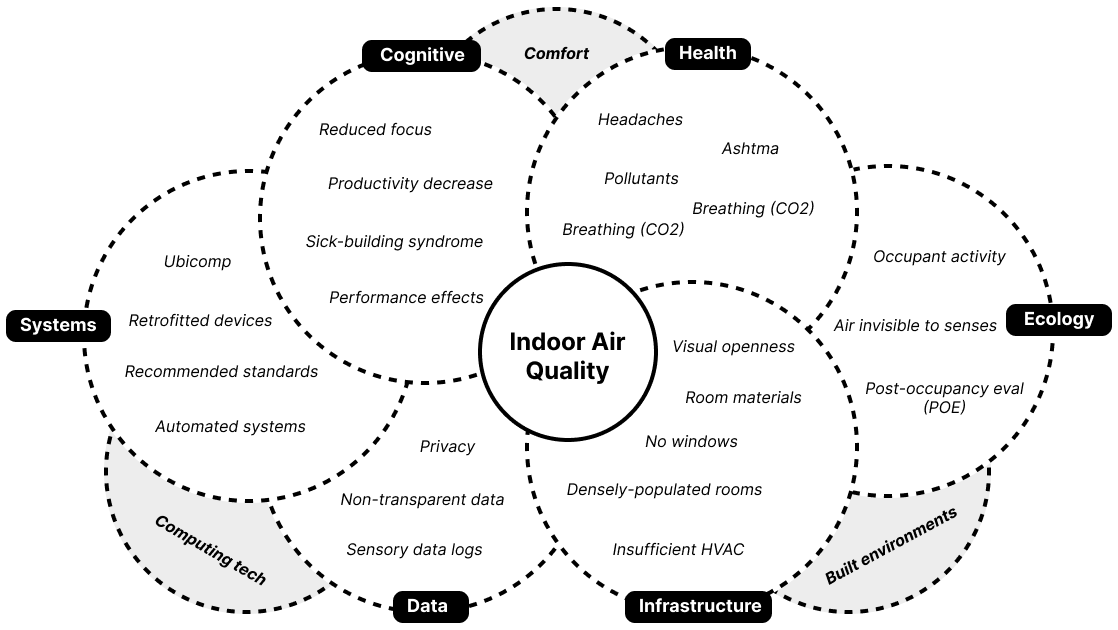
\includegraphics[width=0.47\textwidth]{complexity_diagram_indoor_air_quality.png}
    \caption{Complexity diagram providing an overview of the effects of IAQ and needs of occupants \cite{schweizer_indoor_2007, wang_how_2021, kim_analyzing_2019, alavi_comfort_2017, corlan_importance_2021, klepeis_national_2001}}
    \label{fig:complexity}
\end{figure}


\subsection{Research questions}

In order to research effective ways of communicating  IAQ data, the following main research question is formulated: \\

\emph{RQ: How can real-time sensory measurements and future predictions of indoor air quality be physically visualized to increase awareness among occupants, facilitating their adoption of preventive measures against suboptimal air quality?}\label{rq:1} \\

To effectively answer this central research question, the following supporting sub-questions guide this research and serve as objectives to delineate the necessary knowledge: \\

\begin{enumerate}
    \renewcommand{\labelenumi}{SQ\arabic{enumi}:}
    \item \emph{How aware are occupants of indoor air quality, and how do they understand and perceive its subjective properties?}\label{subq:1}
    \item \emph{How can environmental information related to indoor air quality be incorporated into a physical data-driven representation?}\label{subq:2}
    \item \emph{How do initial experiences of a prototype design solution influence occupants’ awareness of indoor air quality and their willingness to adopt preventive measures?}\label{subq:3}\\
\end{enumerate}
\section{Related Work}
\label{sec:related_work}
Given the focus of this research is studying Human-Computer Interaction (HCI) within Built Environments (BE), this research draws from various related work including the subfield of Human-Building Interaction (HBI) (see \hyperref[sec:hbi]{Section \ref*{sec:hbi}}) and subsequently narrows its focus to Comfort withing Buildings (see \hyperref[sec:poe]{Section \ref*{sec:poe}}) and Indoor Air Quality (IAQ) (see \hyperref[sec:iaq]{Section \ref*{sec:iaq}}) for the scope of this research. Furthermore, it examines notable findings from previous approaches to mapping and encoding sensory data in a new area of research called Data Physicalization (DataPhys) (see \hyperref[sec:phys]{Section \ref*{sec:phys}}).

\subsection{Human-Building Interaction}
\label{sec:hbi}

Buildings increasingly incorporate new forms of digital interaction \cite{pulsipher_towards_2023, margariti_understanding_2023}, which means new inherent connections between 'people', 'built environments', and 'computing' research in an area called Human-Building Interaction (HBI) \cite{alavi_introduction_2019, taherkhani_human-building_2023}. This research area is dedicated to exploring the design of built environments that may incorporate computing to varying degrees \cite{sowles_introducing_2021}.  A logical extension where indoor spaces are increasingly retrofitted with sensing devices \cite{pulsipher_towards_2023}. Understanding how people use different spaces in a building through computing can inform design interventions aimed at improving the utility of the space and the well-being of occupants. \cite{verma_studying_2017}. Current research into architecture and built environments indicates that a significant portion of the data collected by these computing devices is not necessarily transparent or comprehensible to occupants \cite{schnadelbach_adaptive_2019}, and indoor spaces are designed without much thought of placing computing devices integrated within the environment \cite{johansen_temporal_2019, kirsh_architects_2019} leaving users with a perceived lack of control over their indoor comfort. 

\subsection{Comfort within buildings}
\label{sec:poe}

Indoor occupant comfort is achieved in interaction with the environment and is represented in four respective dimensions; thermal, respiratory, visual, and acoustic \cite{alavi_comfort_2017}. Indoor Environmental Quality (IEQ) \cite{kulshreshtha_indoor_2024} indexes serve as metrics for assessing the aforementioned properties of comfort within indoor environments with Post-Occupancy Evaluation (POE) \cite{elsayed_post-occupancy_2023} and Perceived Environmental Qualities (PEQ) \cite{son_perceived_2023} methods being employed to gauge occupants' perceived comfort \cite{boissonneault_concepts_2023}. 

Studies on indoor environments focus on 'static' IEQ conditions using sensors to sense environmental conditions based on the buildings' physical characteristics to meet various recommended standards such as ASHRAE 62.1 \footnote{https://www.ashrae.org/technical-resources/bookstore/standards-62-1-62-2}, ISO 16814 \footnote{https://www.iso.org/standard/42720.html}. Discrepancies between measured IEQ conditions and occupants' perceptions have also been reported in studies. For instance, research indicates that occupants generally have a low awareness of Indoor Environmental Quality (IEQ). While occupants perceive the environment as 'satisfactory', actual sensory measurements within the environment reveal quality levels below recommended standards. \cite{son_perceived_2023}. Recent studies have shifted their focus towards the active role occupants play within the built environment, viewing their behavior within a building as akin to a 'living ecology' \cite{langevin_quantifying_2016} rather than perceiving comfort solely as 'static' properties of the building itself. 


\subsection{Indoor Air Quality}
\label{sec:iaq}

A suboptimal indoor environment has reportedly been associated with health-related problems such as headaches, throat irritation, and asthma \cite{klepeis_national_2001} as well as a decrease in cognitive functions such as tiredness, effects on performance and productivity and a lack of focus \cite{wang_how_2021} \cite{du_indoor_2020}. A phenomenon referred to as the Sick Building Syndrome (SBS) \cite{gawande_indoor_2020, passarelli_sick_2009}. Many of these symptoms are primarily associated with respiratory comfort and are closely tied to Indoor Air Quality (IAQ) concerns \cite{kim_analyzing_2019}. Effective ventilation strategies have been shown to significantly alleviate SBS symptoms \cite{gawande_indoor_2020}.

The advancements of real-time IAQ monitoring systems leveraging Internet of Things (IoT) sensor technology have facilitated progress in both the measurement of IAQ and the implementation of interventions aimed at enhancing it \cite{pantelic_transformational_2022}. Indications of poor air quality are gathered by measuring common pollutants with a focus on molds and allergens (humidity), volatile organic compounds (VOC), and carbon dioxide (CO2) \cite{klepeis_national_2001} where occupant behavior and the number of occupants within indoor space have a specific negative effect on CO2 levels \cite{fromme_indoor_2023}. These indoor climate factors are related to the building occupants’ behaviors and need special attention to be considered in assessing the IEQ conditions and determining if adequate ventilation is present \cite{du_indoor_2020}. It is crucial to recognize that when occupants experience symptoms, it signifies that a suboptimal air quality situation has already occurred.

The existing literature on IAQ offers quantifiable and validated methods for measuring IAQ through sensory data. It underscores the complexities associated with IAQ and emphasizes the significance of developing solutions to ensure occupants receive adequate ventilation.


\subsection{Data Physicalization}
\label{sec:phys}

The research domain known as data physicalization \cite{alexander_data_2019, jansen_opportunities_2015} has emerged as a notable area of study, emphasizing the creation of physical data visualizations making the invisible tangible and interactible by encoding data in physical artifacts \cite{ranasinghe_encoding_2023}. This shift from focusing on individual artifacts to a broader environmental context facilitates the physical embodiment of computing \cite{dragicevic_data_2020}. Data physicalization has the potential to positively influence the perception and exploration of data \cite{jansen_opportunities_2015, wang_emotional_2019, stusak_evaluating_2015}, presenting distinct advantages over traditional 'screen-focused' data representations, such as 2D canvas displays (e.g. digital dashboards) \cite{hornecker_design_2023, jansen_evaluating_2013}, particularly in the context of Indoor Air Quality (IAQ) where a 'physical data visualization' serves as a fitting metaphor for rendering 'invisible' indoor air.These tangible artifacts usually come in the form of ubiquitous computing (ubicomp) \cite{bell_yesterdays_2007} device that seamlessly blends into the environment, essentially making the computing devices 'disappear' \cite{weiser_computer_1999}. 

These devices are frequently employed as persuasive technology, strategically designed to gently nudge individuals towards behavior change leveraging the emerging notion of pervasive sensing to subtly enhance users' awareness regarding the impacts of their decisions \cite{bader_windowwall_2019, rogers_ambient_2010}. This method of persuasive design serves as a powerful tool in calmly extending users' awareness, helping users understand gathered data, and the consequences of their actions, and gaining insight into their behavior \cite{bae_making_2022}. A systematic analysis of over 60 representative data physicalization papers \cite{sauve_physecology_2022} show that only numerous ($f$=3) approaches to studying computing devices within indoor spaces and interactivity with occupants have been explored in prior research especially with a focus on indoor air quality to create awareness and nudge occupants to a desired behavior and rarely on large-scale architectural intervention that is the focus of this research.
This framework of data physicalization and persuasive technology establishes the theoretical foundation for the creation (prototyping) and the evaluation (usability testing) of the design solution within this research.
\section{Methodology}
\label{sec:methodology}

To answer the research question this study uses a human-centered approach (often referred to as Design Thinking) commonly found in Human-Computer Interaction studies consisting of four phases; 1) user studies to \textit{understand} the user, 2) \textit{data collection} methods and analysis of the situation as field trials, 3) \textit{ideation} and experimental design of a prototype and 4) \textit{evaluation} and usability testing of the prototype \cite{jonathan_lazar_research_2017, zimmerman_research_2007}. This mixed-methods approach (both qualitative and quantitative)  helps understand occupants' needs and informs the design and technical set-up of the prototype evaluating the effectiveness by focusing on the user's needs from the start of the study \cite{rogers_moving_2017, experience_ux_2024}. For the first phase, an online questionnaire was conducted to \textit{understand} occupants' awareness of indoor air quality (see \hyperref[sec:questionnaire]{Section \ref*{sec:questionnaire}}), for the second phase a lab setting was created with IAQ monitors to do \textit{data collection} and gain insight into environmental data (see \hyperref[sec:monitoring]{Section \ref*{sec:monitoring}}) which in turn informed phase three the \textit{ideation} and creation of the prototype (see \hyperref[sec:ideation]{Section \ref*{sec:ideation}}, \hyperref[sec:prototype]{Section \ref*{sec:prototype}}). In the last phase participants \textit{evaluated} the prototype and performed usability tests (see \hyperref[sec:evaluation]{Section \ref*{sec:evaluation}}). The concepts of indoor air quality monitoring and data physicalization were investigated through literature review and desk research before setting up the survey, creating the prototype, and conducting the evaluation interviews.

\subsection{Case study building}

This study will be conducted in association with the Digital Interactions Lab \footnote{https://uva-dilab.com/} and will utilize the recently opened Lab42 \footnote{https://lab42.uva.nl/} building at the UvA Amsterdam Science Park \footnote{https://www.amsterdamsciencepark.nl/} as its primary case study location (see \hyperref[appendix:building]{Appendix \ref*{appendix:building}}). Lab42 is an energy-neutral, flexible, and adaptable faculty building that facilitates collaborations among students, researchers, and businesses \cite{benthem_2022}. 

\begin{figure}[H]
    \centering
   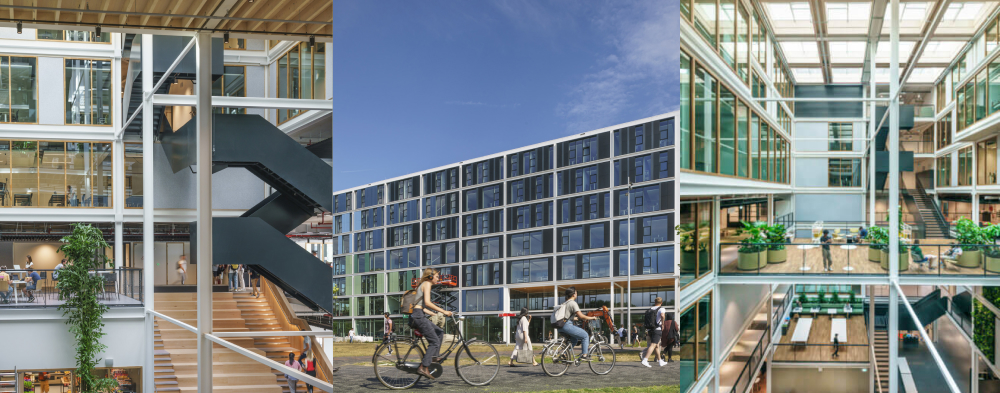
\includegraphics[width=0.45\textwidth,height=0.15\textwidth]{building_impressions.jpg}
    \caption{Impression photographs of the case study building}
    \label{fig:complexity}
\end{figure}

\subsubsection{Space usage}

The buildings's layout is strategically organized into different zones, each serving various functions, ranging from quiet individual work to spaces that allow for collaborative work. Lecture halls, learning rooms, and open learning spaces make up the two lower floors, with the upper four being primarily assigned to the university academic staff, meeting rooms, and external offices. The overarching interior theme in the design revolves around 'tech' and 'nature' aiming to cultivate a fresh, light, and warm comfortable ambiance. Lab42 is an example of a smart building or living lab where sensing devices are retrofitted throughout the building to automatically adjust lighting, temperature, and the focus of this research regulating air \cite{architects_lab42_2022}. This already provides a base of environmental data that can be used and extended for further analysis. Since most of the space within the building is designated as informal learning space and another large part of the building is designed as meeting rooms (see \hyperref[appendix:meetings]{Appendix \ref*{appendix:meetings}}), working areas these functions of focussed work and collaborative meetings can be heavily influenced by reduced cognitive performance as a result of poor indoor air quality.

\subsection{Questionnaire survey}
\label{sec:questionnaire}

To understand and collect occupants' subjective awareness and satisfaction of IAQ a structured survey was created to gather quantitative data within the building as a form of Post Occupancy Evaluation (POE) (see \hyperref[appendix:survey]{Appendix \ref*{appendix:survey}}).


\subsubsection{Questions}
The questions were based on two POE studies with a focus on indoor air quality \cite{silva_post-occupancy_2017, son_perceived_2023} and used standardized questions (e.g. Q-bank) and scales (e.g. Likert-scale) similar to Customer Satisfaction (CSAT) surveys. The survey consisted of a total of 9 questions (5 multiple choice, 3 Likert scales, 1 not mandatory open question) consisting of questions about:

\begin{enumerate}
  \item \textit{Activity and occupancy:} the rough location the occupant is within the building, how often the occupants use the building for various activities, and how they would describe the occupancy in their current space.
  \item \textit{Awareness and satisfaction:} how aware the occupant is of the current air quality in the space, how the occupant perceives the air quality in the current space, and how satisfied the occupant is with the air quality in the current space.
  \item \textit{Health and cognitive symptoms :} if the occupant experiences any health or cognitive symptoms based on the air quality in the current space.
\end{enumerate}


\subsubsection{Participants}
The survey was distributed via handouts with QR Codes using eligibility criteria based on demographic characteristics to occupants present at the informal learning spaces of the atrium, first floor, and second floor. There were no additional inclusion criteria besides the convenience sampling size of respondents being present in the case study building (sampling in context). Additionally, handouts were attached to the tables using stickers. All instances of participation were voluntary and conducted without remuneration. Distribution of the survey was open for submission from the 1st of March to the 31st of April 2024 which recorded X ($n$=X) responses in total of which after cleanup a total of X ($n$=X) responses were included in the final dataset. No personally identifiable information such as age and gender was collected during the survey and ethical considerations (e.g. consent forms) were taken into consideration. To improve the quality of the questionnaire on the initial version feedback was requested, after which the survey protocol was piloted, before distributing to participants (see \hyperref[appendix:experts]{Appendix \ref*{appendix:experts}}). 

\subsubsection{Data cleaning, preprocessing and analysis}
\label{sec:analysis}
After the distribution of the survey completed analysis of the collected data was performed in the form of data cleanup and exploratory data visualization. In Python (Jupyter Notebook format) \footnote{https://jupyter.org/} Libraries such as Numpy \footnote{https://pandas.pydata.org/} were used to clean the data (e.g. remove non-consenting users) and visualization libraries such as Seaborn \footnote{https://seaborn.pydata.org/} were used to create graphs and plots (e.g. boxplot the likert-scales) to get an overview of the collected data and gain insight into understanding the occupants.

\begin{figure*}[!t]
    \centering
    \begin{subfigure}[b]{0.23\textwidth}
        
\includegraphics[width=\textwidth]{placeholder.jpg}
        \caption{Placeholder caption}
        \label{fig:1}
    \end{subfigure}
    \hfill
    \begin{subfigure}[b]{0.23\textwidth}
        
\includegraphics[width=\textwidth]{placeholder.jpg}
        \caption{Placeholder caption}
        \label{fig:2}
    \end{subfigure}
    \hfill
    \begin{subfigure}[b]{0.5\textwidth}
        
\includegraphics[width=\textwidth, height=0.46\textwidth]{placeholder-two.jpg}
        \caption{Placeholder caption}
        \label{fig:3_4_combined}
    \end{subfigure}
    \caption{Impressions of the ideations and prototyping phase}
    \label{fig:full_width}
\end{figure*}

\subsection{Air Quality Monitoring}
\label{sec:monitoring}

To gather data about the current situation of air quality within the building and understand the current situation within the building in terms of air quality data we retrofitted IAQ monitors to two specific meeting rooms within the building (see \hyperref[appendix:floorplan]{Appendix \ref*{appendix:floorplan}}). This data collected was further used to inform and acted as a basis for the data input of the data physicalisation (see \hyperref[sec:prototype]{Section \ref*{sec:prototype}}).

\subsubsection{Technical set-up}

We deployed the monitors in meeting rooms occupants regularly use which allowed us to understand occupants' behavior and perception in real-world corporate settings as opposed to a controlled lab setting. We refer to them as the small room (room A) and the large room (room B). The small room is XX m2 and is commonly used for small-size meetings (seven seats), while the large room is XX m2 (fourteen seats), which is preferable for hosting larger-size meetings and seminars. Two commercially available indoor climate data loggers were installed using 3D printed mounting plates, an AirCheq Touch Aero \footnote{https://airteq.eu/producten/touch-aero/} in the smaller room and an Atal ATU-CT ClimaTrend \footnote{https://www.atal.nl/atu-ct-climatrend-binnenklimaat-datalogger} in the larger room. Both monitors use industry-standard (e.g. Senseirion and SenseAir) sensors to measure common pollutants and were mounted (e.g. between 80cm and 120cm from the ground) and calibrated (e.g. intervals, polling rates) as described by both manufacturer's installation manuals. The monitoring devices were installed from the 1st of March to the 31st of April 2024

\begin{table}[htbp]
    \centering
    \caption{Subset sample data of the IAQ monitors}
    \begin{tabular}{lccc}
        \toprule
        \textbf{Time} & \textbf{Humidity (\%)} & \textbf{VOCs (ppm)} & \textbf{CO2 (ppm)} \\
        \midrule
        08:00 & 40 & 0.05 & 500 \\
        09:00 & 42 & 0.06 & 520 \\
        10:00 & 45 & 0.07 & 550 \\
        \bottomrule
    \end{tabular}
    \label{tab:air-quality}
\end{table}

\subsubsection{Data logs}

The data gathered by the sensors provides insights into various standardized measurements related to common pollutants that affect IAQ such as molds and allergens (humidity), volatile organic compounds (VOC), and carbon dioxide (CO2) (see \hyperref[tab:air-quality]{Table \ref*{tab:air-quality}}, \hyperref[appendix:monitors]{Appendix \ref*{appendix:monitors}}). We cross-referenced the data logs with weekly schedules based on the internal booking systems of the rooms based on the timestamped data to align the values of the sensors from the data logs when meetings were scheduled. Data analysis is performed similarly as described in (see \hyperref[sec:analysis]{Section \ref*{sec:analysis}}). were data was cleaned to remove data from mainly non-opening hours and plotted and visualized to explore patterns in the data and cross-reference them with meeting times.


\subsection{Ideation and requirements}
\label{sec:ideation}

As a starting point for creating a physical representation of the air quality data we base our formative research on the growing interest in establishing theoretical and design foundations for \textit{data physicalisation} \cite{hornecker_design_2023, sauve_physecology_2022, bae_making_2022} on how to encode the properties and use a common design language \cite{ranasinghe_encoding_2023, sosa_data_2018} established by systematic reviews of data physicalization projects. The creation of a prototype illustrates the technology to be and are often deployed to conduct lab experiments and case studies \cite{jonathan_lazar_research_2017}. The overall goal of the physicalization is described in the following definition:

\AtBeginEnvironment{quote}{\setlength{\leftmargini}{10pt}}
\AtBeginEnvironment{quote}{\itshape}
\begin{quote}
a data-driven physical artifact whose geometry and material properties encode data that aims to augment a nearby audience’s understanding of data insights.
\end{quote}

The goal of the prototype is to generate knowledge about the intervention and human behavior around it. This is in alignment with a pragmatist methodology in design research where methods are adapted and evolve through interactions with participants. Before prototyping the design solution we first describe the overall requirements and scope of the physicalization and case studies used for ideation. The final prototype is described based on the encoded variables and design dimensions found in the literature (see \hyperref[sec:prototype]{Section \ref*{sec:prototype}}).

\subsubsection{Concept requirements}

Based on this scope and the survey we describe the concept requirements ("r" for "requirements") of the design solution in further detail with six overarching requirements ranked based on the Moscow method:

\begin{enumerate}
    \renewcommand{\labelenumi}{R\arabic{enumi}:}
    \item \textbf{Visual Feedback:} The prototype must provide visual feedback through movement encoding environmental properties that represent air quality metrics, ensuring that users can easily interpret the information conveyed (must have).
    \item \textbf{Size and location:} The prototype must be designed to be installed within small to medium-sized rooms, with consideration for its dimensions and weight to ensure compatibility (must have).
    \item \textbf{Real-Time Data Integration:} The prototype should integrate real-time data from air quality monitors to dynamically adjust its behavior (should have).
    \item \textbf{Interactive sensing:} The prototype should be interactive in which occupants can interact with the prototype by walking near it providing a tactile experience (should have).
    \item \textbf{Material durability:} The prototype could use natural materials and be durable and resistant to environmental factors such as humidity and temperature fluctuations (could have).
    \item \textbf{Aesthetic Integration:} The prototype could seamlessly integrate with its surrounding environment, complementing interior design aesthetics, architectural features, and layouts of the room to enhance the overall ambiance (could have).
\end{enumerate}

\subsubsection{Concept models}

For the concept models, two existing datasets of academic and non-academic case studies were used as comparative studies, desk research, and as a starting point for ideation. First was the DataPhys gallery \footnote{http://dataphys.org/list/gallery/}, a collection of 372 entries classified as data physicalizations. The second was a combination of three state-of-the-art papers with systematic reviews of physicalization with combined examples of around 132 entries classified as data physicalization of which both academic and non-academic samples \cite{sauve_physecology_2022, anhalt_university_germany_design_2022, ranasinghe_encoding_2023}. Out of these, seven ($f$=7) samples of academic were selected for further review based on the similarity with the before described requirements of which three ($f$=3) samples with a focus on the environmental property of air, but not necessarily air quality within indoor environments (see \hyperref[appendix:academic]{Appendix \ref*{appendix:academic}}). Additionally, fifteen ($f$=15) samples of non-academic case studies were reviewed after desk research which included work and prototypes from design studios and independent creators that informed the ideation phase (see \hyperref[appendix:nonacademic]{Appendix \ref*{appendix:nonacademic}}).

\subsubsection{Concept diagrams}

Based on the user requirements and ideation and concepting from the Communication and Multimedia Design (CMD) Methods Pack \footnote{https://cmdmethods.nl/} and Design Method Toolkit \footnote{https://toolkits.dss.cloud/design/} by the Digital Society School (DSS) three low fidelity (lo-fi) concepts were further elaborated (see \hyperref[fig:3_4_combined]{Figure \ref*{fig:3_4_combined}}) in order to choose one to develop in high fidelity (hi-fi) for the user studies and evaluation. 

Concept selection was based on weighted physicalization criteria from the literature, a Harris profile for the lo-fi concepts, and four expert reviews ($n$=2 internal experts involved in the project, $n$=2 external experts not involved in the project) feedback (see \hyperref[appendix:profile]{Appendix \ref*{appendix:profile}}, \hyperref[appendix:expert]{Appendix \ref*{appendix:expert}}). Also technical limitations of the provided hardware (e.g. real-time data output of monitors, cost of hardware, availability of electronic components,) and limitations in the technical set-up of the building (e.g. space in the meeting rooms, not allowed to alter furniture) were considered as heuristic evaluation. Based on the aggregation of these criteria the \textit{Bluebird} concept was chosen to be further developed into a high-fidelity prototype (see \hyperref[fig:bluebird]{Figure \ref*{fig:bluebird}}, \hyperref[appendix:prototype]{Appendix \ref*{appendix:prototype}}).

\subsection{Evaluation}
\label{sec:evaluation}

The prototype was evaluated as summative research using common performance-related criteria that are widely used in HCI/Information Visualisation \cite{ranasinghe_encoding_2023} and Grounded Theory studies \cite{chun_tie_grounded_2019}. We employed a field-based evaluation approach with accompanying methods based on the Human-centered Design Kit by Ideo \footnote{https://www.designkit.org/methods.html} and Delft Design Guide from the Delft University of Technology (TU) \footnote{https://www.bispublishers.com/delft-design-guide-revised.html}. For evaluation criteria, we used the intentions and evaluating interview methodology described in the data physicalization design vocabulary \cite{jansen_evaluating_2013,ranasinghe_encoding_2023} as a baseline for evaluating the learnability, memorability and usefulness using in-person evaluation sessions. To measure these properties of understanding and usability of the data physicalization we adopted and rewritten questions from the Technology Acceptance Model (TAM), Software Usability Measurement Inventory (SUMI) and System Usability Scale (SUS) to gather insight into perceived usefulness, attitude towards using, and system usability\cite{davis_perceived_1989, brooke_sus_1996}. These questions acted as a baseline and starting point but where revised and remixed to suit the specifics of evaluating data physicalizations within the context of this research (see \hyperref[appendix:evaluation]{Appendix \ref*{appendix:evaluation}}).

\subsubsection{Hypothesis elicitation}

Based on the research question and creation of the prototype three hypotheses ("h" for "hypothesis") were formulated to evaluate as an observational study:

\begin{enumerate}
    \renewcommand{\labelenumi}{H\arabic{enumi}:}
    \item \textbf{Understanding:} users will exhibit a clear comprehension of the physicalization's representation of IAQ data, as well as an understanding of its intended function and impact
    \item \textbf{Self-reflection:} users exposure to real-time IAQ data visualizations through the prototype will prompt users to reflect and will lead to increased awareness.
    \item \textbf{Effectiveness:} users acceptance and satisfaction with the IAQ physicalization will be positively correlated with perceived usefulness, attitude towards use, and system usability.
\end{enumerate}

\subsubsection{Participant sampling}

The sample size of evaluation interviews was x ($n$=X) and accepted because the study findings reached theoretical saturation, new interviews did not yield new insights after the first x interviews and led to repetitive data \cite{steph_menken_introduction_2016}. Participants were gathered through purposive sampling and recruited through internal communication of the studies via email and internal lab messaging tools. The participants were not involved in the development of the prototype and had no prior knowledge of the purpose of the prototype and its design of it. Participants were not (financially) incentivized to take part in the studies. Respondents had to meet the inclusion criteria ("c" for "criteria") that needed to be checked before the interviews: 

\begin{enumerate}
    \renewcommand{\labelenumi}{C\arabic{enumi}:}
    \item The participant needed to use a meeting room with the building a minimum of once a week
    \item The participant needed to work within the case study week a minimum of 3 days per week
\end{enumerate}

This resulted in a sample of x male, x female, consisting of various roles; from researchers from different labs, PhD candidates working at the labs to private company employees encompassing a range of ages ($min$=x, $max$=x, $mdn$=x) and education levels. Participants used the meetings rooms on average x ($min$=x, $max$=x, $mdn$=X) a week and worked within the lab42 building x ($min$=x, $max$=x, $mdn$=X) a week. The evaluation session where held between May 1st to 31st of May 2024

\subsubsection{Evaluation interviews}

Within the meeting-room lab set-up in the presence of the developed prototyped pre-arranged, semi-structured individual qualitative interviews were conducted with open-ended and nonleading questions with additional in-depth questions (follow-up probing strategy) on topics emerging from the dialogue (see \hyperref[appendix:evaluation]{Appendix \ref*{appendix:evaluation}}). To improve the quality of the interviews (and evaluation session in general) on the initial version feedback was requested, after which the interview protocol was piloted, before continuing with participants (see \hyperref[appendix:experts]{Appendix \ref*{appendix:experts}}). The goal was to gather first impressions and gain insight into how occupants understand the communicated data factors of the prototype. Some questions were purposefully vague to explore how the building occupants understand and use the prototype. Also in these cases the purpose of the prototype was not communicated to participants before-hand to gather first impressions.

\subsubsection{Participant observation (usability testing)}

After the explorative questions participants were encouraged to in more detail view the prototype and interact with it as a field trial stating anything they noticed (encouraging probing strategy). Participants' behavior was observed within prolonged engagement in the meeting rooms and participants were encouraged to think aloud when viewing and interacting with the prototype (see \hyperref[appendix:usability]{Appendix \ref*{appendix:usability}}). Informal leading questions were asked about improvements, design optimization, and visual changes. In this manner, insights into particular interaction elements were acquired without the explicit involvement of HCI specialists. The goal was to test the usability of the prototype, study occupants and their behavior in a natural setting, and gather insight into the self-reflective properties of the prototype. 

\subsubsection{Prototype effectiveness}

After the interviews and observations, the participants were asked to fill in a digital online with structured pre-defined questions form rating several properties of the prototype for their effectiveness (see \hyperref[appendix:effectiveness]{Appendix \ref*{appendix:effectiveness}}). The goal was to gather quantitative measurements about the usability and effectiveness of the prototype.

\subsubsection{Transcription and coding}
All interviews were anonymized and conducted in-person on-site and audio recorded with permission of the participants. The recordings were then verbatim transcribed using the built-in Microsoft 365 transcription tool \footnote{https://www.microsoft.com/nl-nl/microsoft-365} to avoid bias while note-taking. The transcribed interviews as textual data were processed via Atlas.ti \footnote{https://atlasti.com/} for qualitative coding.

\begin{figure*}[b]
    \centering
        \begin{subfigure}[b]{0.45\textwidth}
        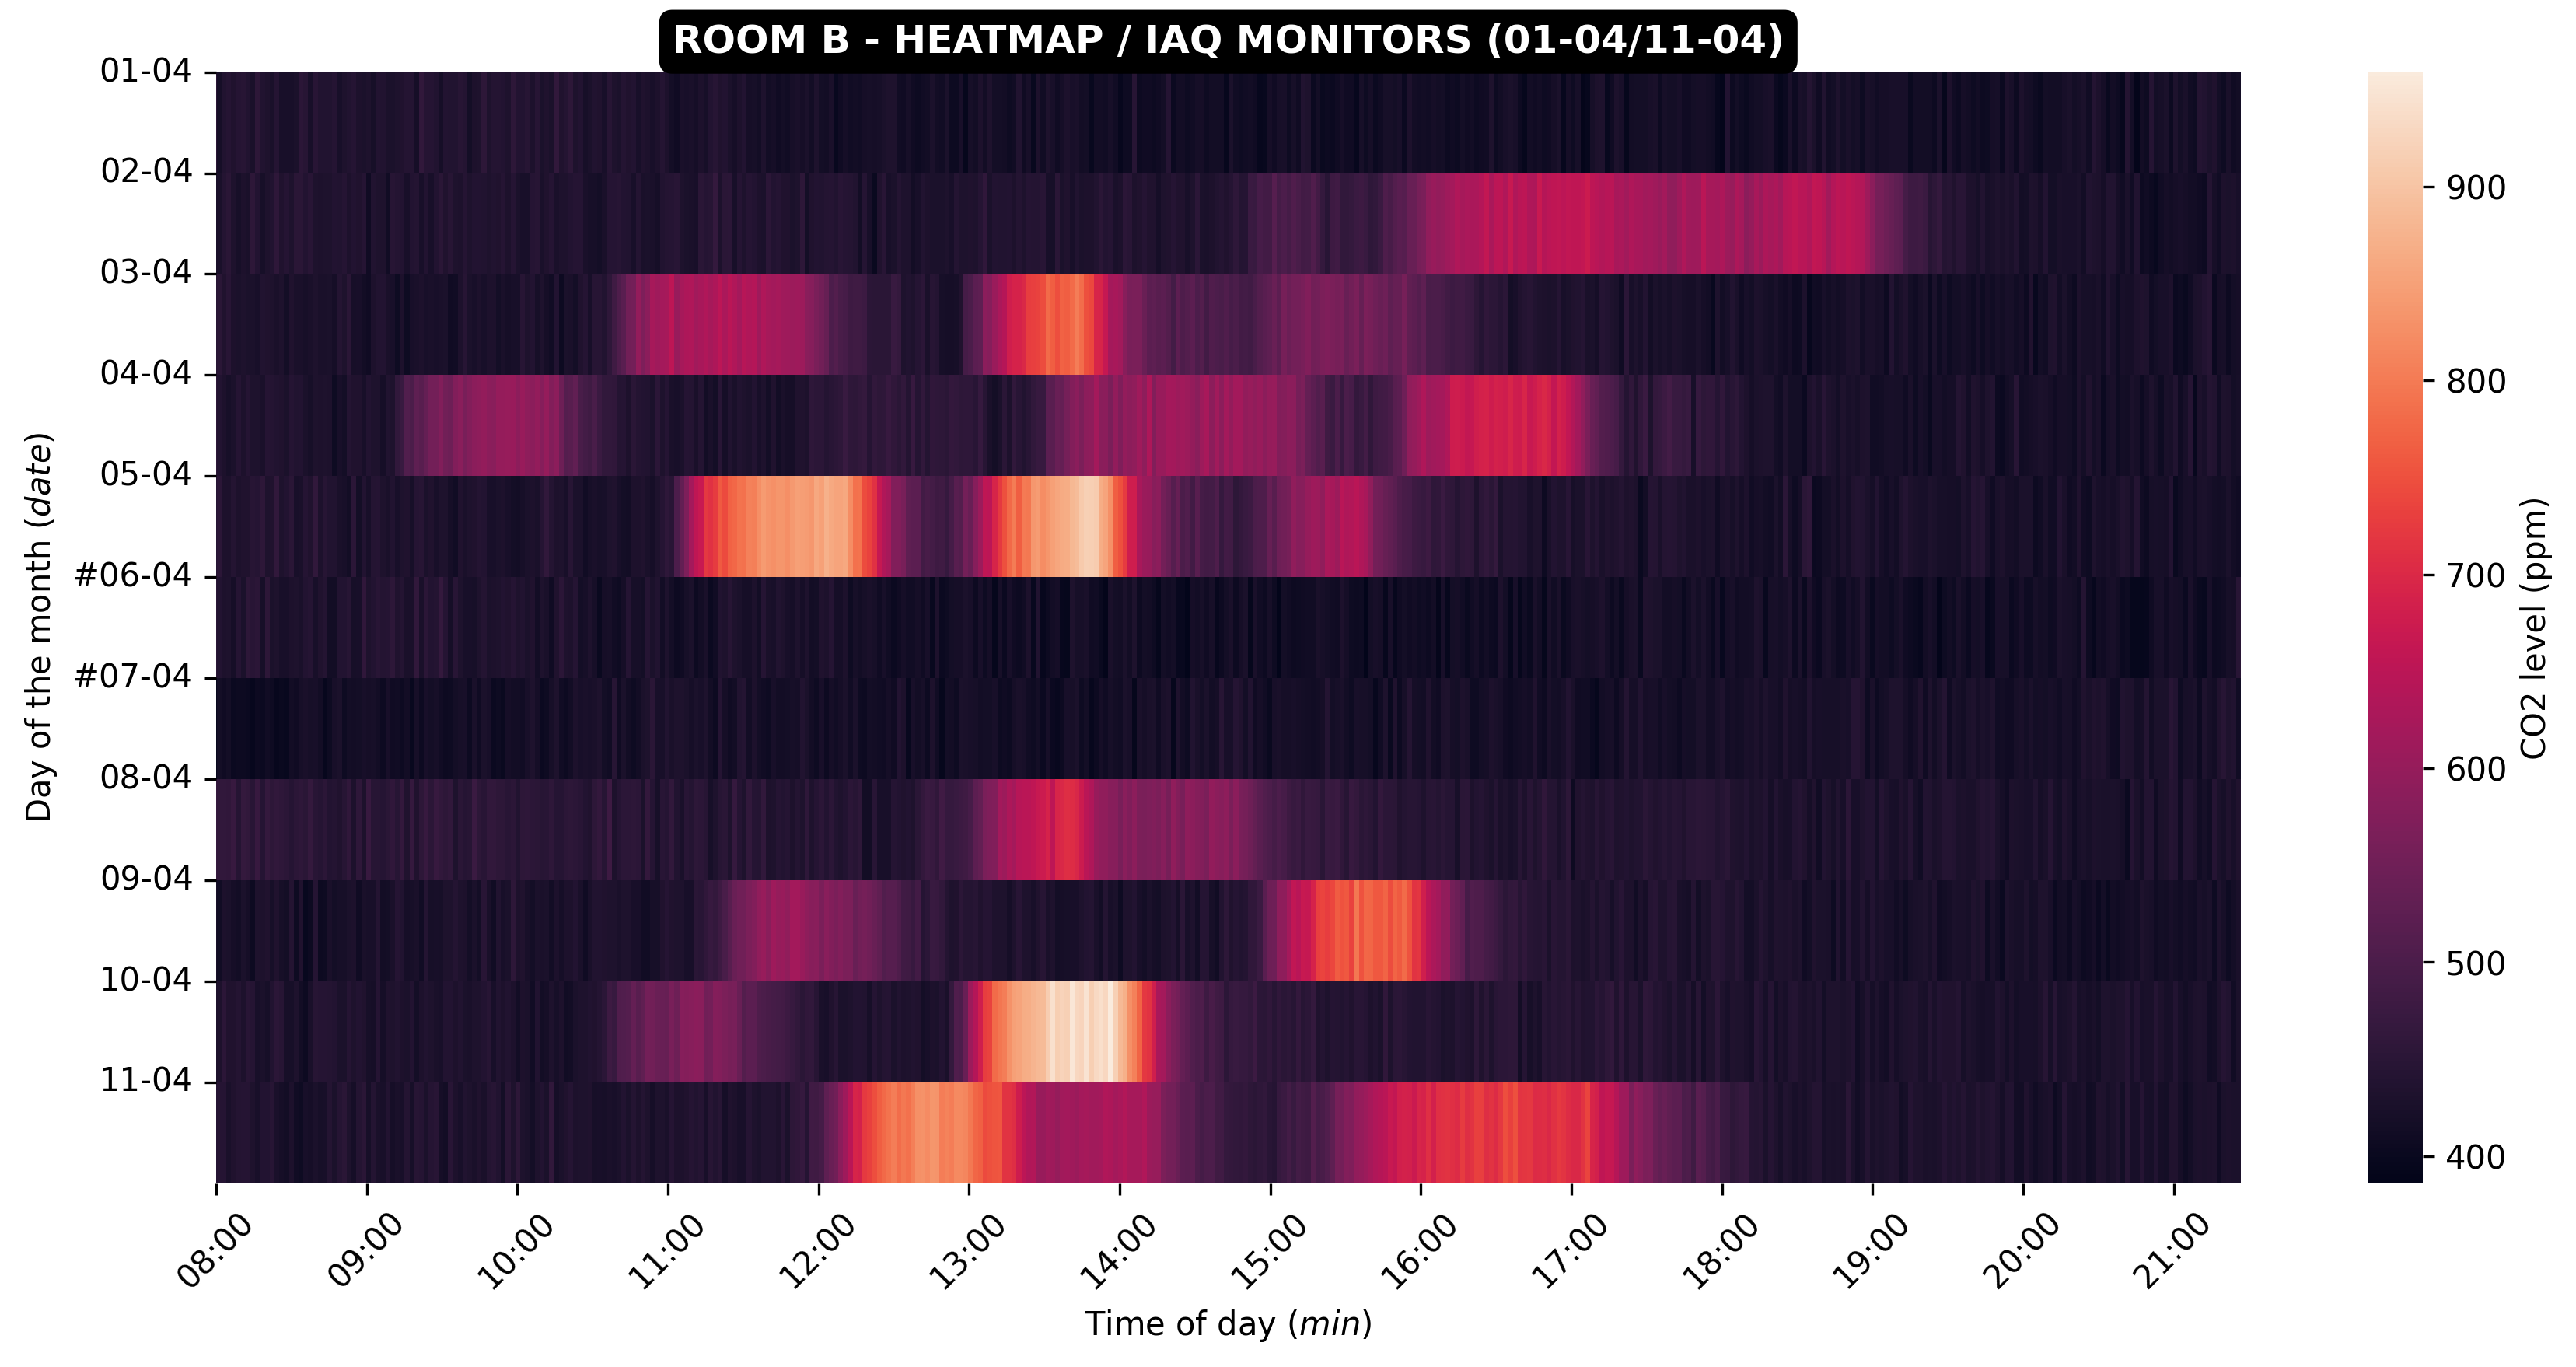
\includegraphics[width=\textwidth]{room-b-monitor-heatmap.png}
        \caption{Heatmap of Room B with ten days of data collection}
        \label{fig:3_4_combined}
    \end{subfigure}
    \begin{subfigure}[b]{0.5\textwidth}
        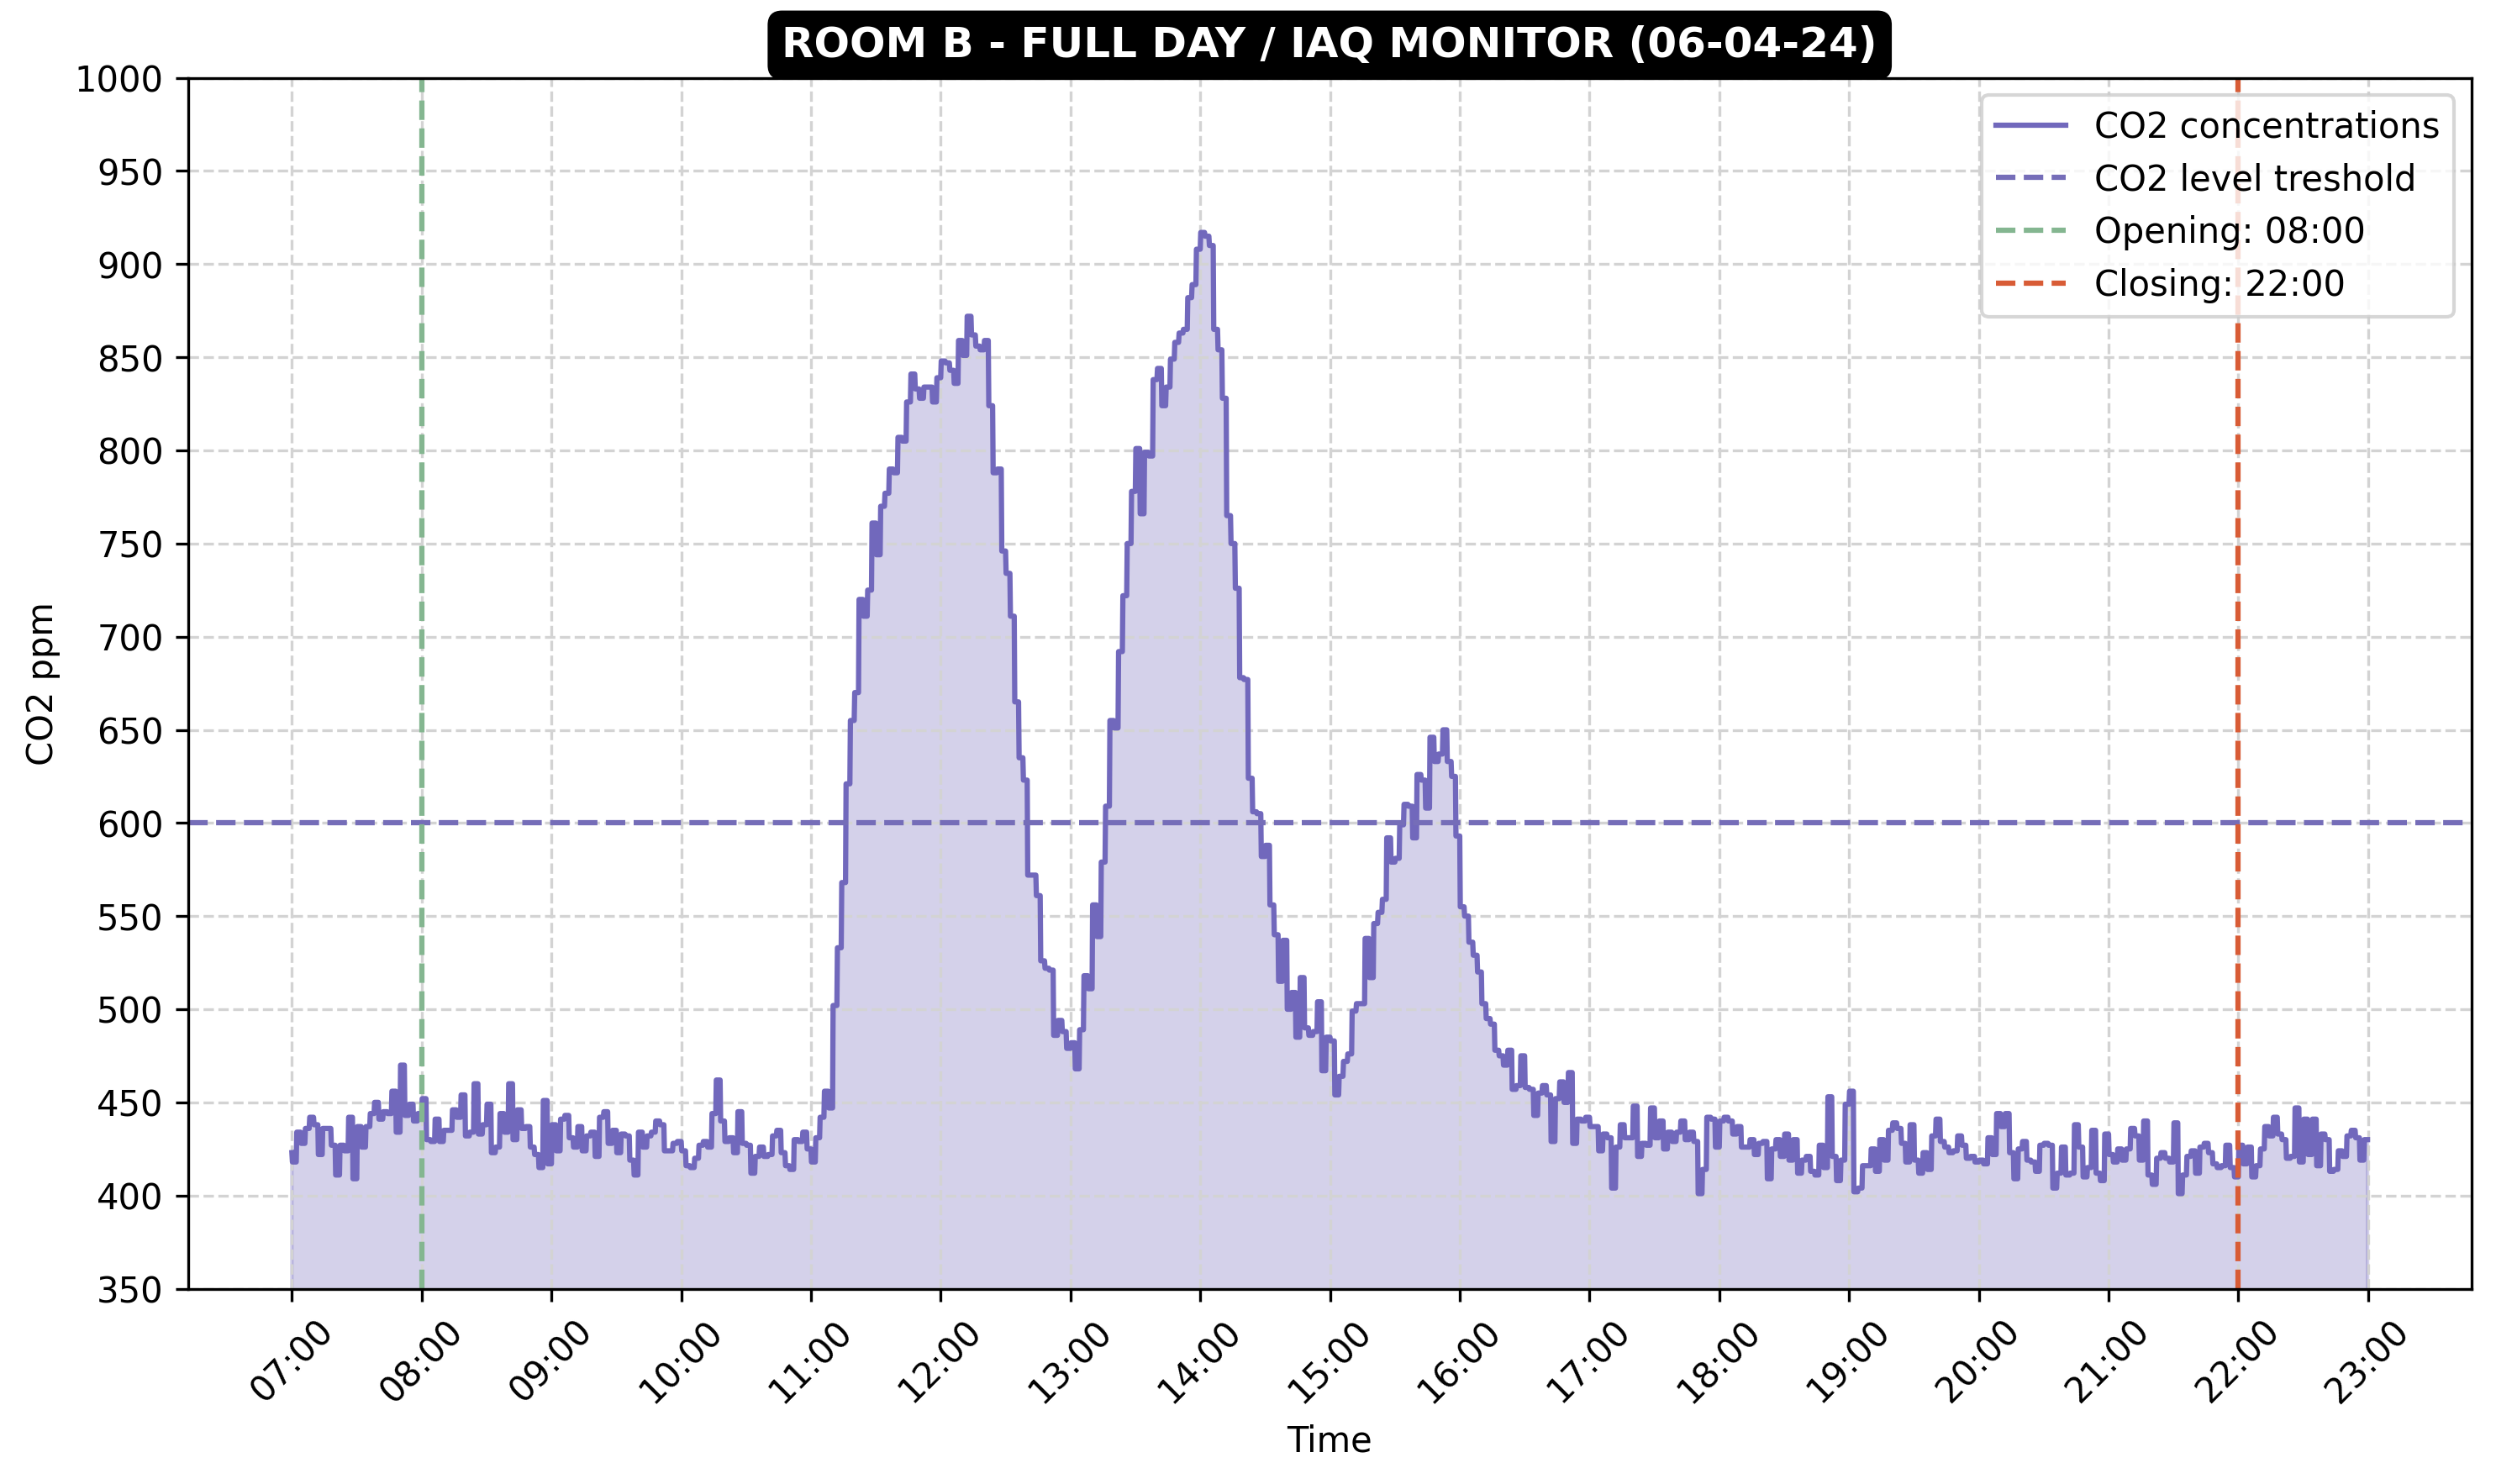
\includegraphics[width=\textwidth]{room-b-monitor-meeting-spike-day.png}
        \caption{Lineplot of Room B with a single day of meetings}
        \label{fig:1}
    \end{subfigure}
    \hfill
    \caption{Plots of the IAQ monitor data logs CO2 concentrations within the meeting rooms}
    \label{fig:full_width}
\end{figure*}
\section{Results}
\label{sec:results}

The goal of the chosen methodologies (see \hyperref[sec:related_work]{Section \ref*{sec:related_work}}) allows for answering of the \hyperref[rq:1]{(sub)research questions}. First, the results of the questionnaire survey are described (see \hyperref[sec:survey_analysis]{Section \ref*{sec:survey_analysis}}) and key insights into the air quality monitor data collection are presented (see \hyperref[sec:monitor_analysis] {Section \ref*{sec:monitor_analysis}}) to answer \hyperref[subq:1]{SQ\ref*{subq:1}}. Then the developed prototype will be presented in section (see \hyperref[sec:prototype_results]{Section \ref*{sec:prototype_results}}) which addresses \hyperref[subq:2]{SQ\ref*{subq:2}} and the results from the evaluation sessions will be summarized in (see \hyperref[sec:evaluation_results]{Section \ref*{sec:evaluation_results}}) to address \hyperref[subq:3]{SQ\ref*{subq:3}}.

\subsection{Survey analysis}
\label{sec:survey_analysis}

The following section presents the outcomes of the survey conducted to assess various aspects related to occupants' activity, IAQ awareness, satisfaction, perception, and health impacts among Lab42 building occupants. The responses show that most occupants are located in the atrium of the building, not particularly aware of the IAQ, and perceive the IAQ as acceptable based on the large open area and planters, meeting satisfactory IAQ levels.

\begin{figure}[H]
    \centering
    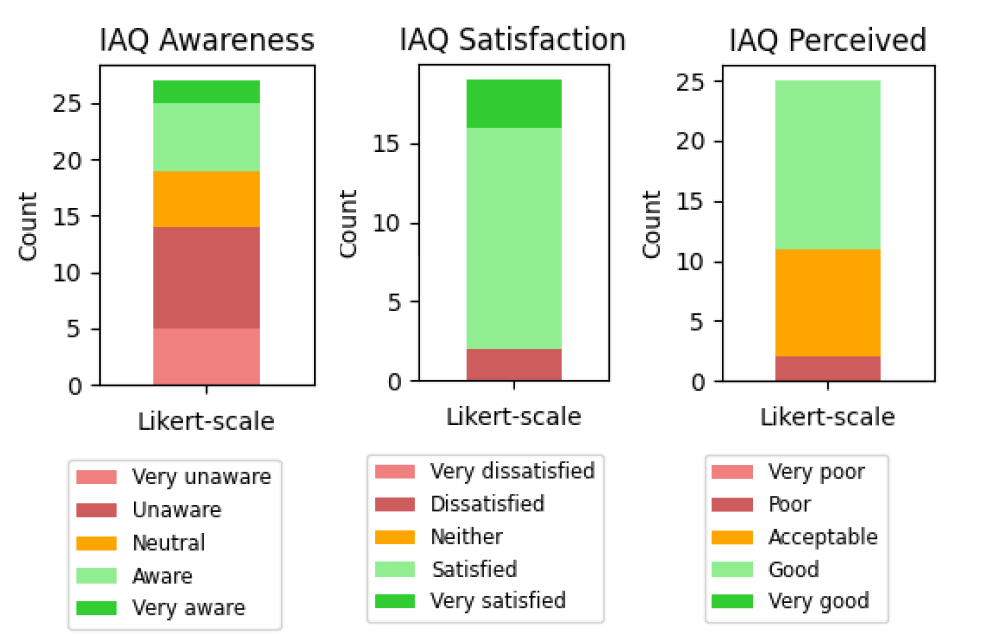
\includegraphics[width=0.5\textwidth]{IAQ_LIkert-Scales_Survey.jpg}
    \caption{Likert-scales of IAQ awareness, perception and satisfaction of the questionnaire survey with occupant count}
    \label{fig:complexity}
\end{figure}

\subsubsection{Activity and occupancy}

The first set of questions of the survey focussed on activity and occupancy. On average, occupants who filled in the survey used the Lab42 building \textit{3 times a week} for various activities ($f$=X). As opposed to 1 day a week, 4 days a week, 2 days a week with a small number of occupants using the building 5 days a week. Most occupants from the sample size were located on the \textit{ground floor ($f$=X) and the first floor ($f$=X)} as opposed to the 2nd floor. Both the first floor and ground floor are considered the 'open area' and part of the atrium of the building. This is by design of the building where the lower floors have more co-working spaces to be used as informal open learning spaces whereas the upper floors are more designed as meeting rooms and private working offices. Many occupants described the overall occupancy in the space as \textit{not too crowded} ($f$=X) with a smaller percentage explicitly stating the space was crowded or not crowded at all.

\subsubsection{Awareness, perceived and satisfaction}

The second set of questions were three Likert scales about perceived IAQ, awareness of IAQ, and satisfaction with IAQ. Over half of the occupants are \textit{not particularly aware} of the IAQ in their current space, either very unaware ($f$=X), unaware ($f$=X), or neutral ($f$=X) the minority of the occupants are aware or very aware. Indicating that in general occupants are not very aware of the IAQ if they are directly asked about it. However, once occupants are asked about their perceived IAQ and satisfaction the majority of the occupants perceive the IAQ as \textit{acceptable ($f$=X) or good ($f$=X)} and almost all occupants consider the IAQ as satisfactory by being \textit{satisfied ($f$=X) or very satisfied ($f$=X)} with the IAQ.

\subsubsection{Health and cognitive symptons}

The third set of questions were to indicate if users suffered from health or cognitive symptons based on the IAQ. The majority of participants answered \textit{none} to both the health ($f$=X) and cognitive ($f$=X) questions. A small percentage experienced health symptoms such as headaches and feeling noiziating and a larger percentage experienced cognitive symptons such as trouble with focus or tiredness. The results of this section of the survey are inconclusive since it's difficult to determine if these symptons are specifically related to the air quality.

\subsubsection{Open-ended air quality description}
The most notable finding of the open question is that the occupants who filled in the not mandatory question describing their perception of IAQ mention specifically the openness of the atrium space:

\begin{quote}
P11: "[...] think it is good, [...] although I must say that this is mostly based on the large amount of open space in the building"
\end{quote}

With some of the occupants mentioning the 'high ceilings' of the atrium specifically.

\begin{quote}
P8: " [...] feel like in this building the air quality is really good, mainly because of the impression the high ceilings give"
\end{quote}

\begin{quote}
P13: "I like the air quality. This may also be because I sit close to the door and the ceiling is high."
\end{quote}

Another notable attribute is that many occupants describe contributing to the perception that the IAQ is sufficient are the hanging planters and greenery that is present within the atrium.

\begin{quote}
P16: "[..] I also see green plants around me, of which I think they are real."
\end{quote}

\begin{quote}
P14: "[...] and the hanging plants that are present.
\end{quote}



\subsection{Air Quality Monitors}
\label{sec:monitor_analysis}

The gathered data logs are exported from the devices and analyzed with a focus on CO2 concentrations since this is the main IAQ parameter that influences air quality negatively within indoor environments based on occupancy within a room. Analyzation of the data logs shows occupancy patterns of a 'typical meeting', scheduled meeting patterns for the case study rooms and more notably the development of CO2 concentrations within both meeting rooms regularly where they regulary exceed optimal CO2 concentration tresholds above 600ppm.

\subsubsection{Single meeting CO2 development}

A sample of CO2 concentrations in a single meeting is shown in (see \hyperref[fig:complexity]{Figure \ref*{fig:complexity}}). The lineplot shows the development of a 'regular' 1-hour meeting within the room. The plot are the CO2 concentrations over time in minutes with a x-axis line of 600ppm indicating the maximum 'ideal' treshold. Two coloured lines on the y-axis indicate the start and end time of the meeting. The observations show that after 15 minutes of the meeting started the CO2 concentrations reach suboptimal levels and continou to rise towards 950ppm level where it stabilizes as the 'maximum value' of the meeting. As stated before, continous exposure to CO2 concentrations especially between 800ppm - 1000ppm and even above are considered 'bad' and can impact cognitive functions. After ending of the meeting the concentrations slowly start to decrease to the baseline of 450ppm when occupants leave the meeting room at the end time.

\subsubsection{Regular day CO2 development}

The visualization (see \hyperref[fig:complexity]{Figure \ref*{fig:complexity}}) shows the spikes of CO2 concentrations during a sample day where multiple meetings occured. Again, the x-axis plots the CO2 concentrations and this time the y-axis shows a full day with opening hours of the building. Based on similar plots of randomly sampled days the data shows most meetings occur between late in the morning (11:00) and usually end late in the afternoon (17:00) where after no more meetings are planned. That's roughly two hours after opening of the building and roughly four hours before closing of the building. There are outliers, on some days meeting occur early in the morning straight after opening time, and occassionaly a (longer) meeting that is longer and spans longer in the evening.

\subsubsection{Meeting schedule CO2 development}

A heatmap of ten days of CO2 concentration monitoring (see \hyperref[fig:complexity]{Figure \ref*{fig:complexity}}) shows that it's common that two or three meetings occur on a single day and typically spans one hour. The majority of the meetings go beyond the 600ppm CO2 concentrations. Based on the lineplots and heatmaps it is assumed that the 'larger' Room B is more frequently used and reaches higher CO2 concentrations but those results are not definite since it heavily relies on context and the dates and time periods that spanned the data collection and the monitors were installed.

\subsection{Prototype}
\label{sec:prototype_results}

Based on the requirements, data physicalization design principles, and concept models exploration a final high fidelity (hi-fi) version of the prototype was developed that functioned as a proof-of-concept of the physical design solution as a feasibility study and utilized in the user study for evaluation.

\subsubsection{Concept description}

\textit{Bluebird} is a hanging kinetic type sculpture inspired by organic nature materials and the shapes of hanging planters that encode the environmental properties of indoor air quality data. It is meant to be hung from the ceiling in small to medium rooms and changes based on real-time air quality monitor data. Strings (plant branches) either become longer or smaller simulating the growth of a plant. Movements of the leaves indicate the freshness of air and movement. The overall design philosophy of the shapes and forms uses the notion of calm technology to minimize interruption cost \cite{case_calm_2016}. 

\subsubsection{Electronics and components}

A controller device running on an Arduino Uno R3 \footnote{https://store.arduino.cc/products/arduino-uno-rev3} microcontroller with an MKR Motor shield is used \footnote{https://store.arduino.cc/products/arduino-motor-shield-rev3} to control six 360° MG90S type Micro Servo Motors \footnote{https://www.towerpro.com.tw/product/mg90s-3/}. Attached to these motors are pulleys with fishing lines simulating the growth of the hanging planter so that the string can be moved up and down.


\subsubsection{Crafting technologies and materials}
The strings, leaves, and housings of the electronics and mechanical hardware are created using additive manufacturing (3D Printing) using a Fused deposition Modeling (FDM) technique using Polylactic acid (PLA) plastic filament in various colors. The electronics enclosures and plant models were modeled using computer-aided design (CAD) software. A digital fabrication technique commonly found in data physicalization prototypes \cite{anhalt_university_germany_design_2022}. To create leaves representing textile or fabric custom properties were defined within the 3D printing software (Slicing) to remove top and bottom layers and create a thin layer of infill.

\subsubsection{System Architecture and software}

The microcontroller uses custom firmware written in Arduino code \footnote{https://www.arduino.cc/reference/en/} (similar to C++) that receives real-time data from the air quality monitors using the LoRaWAN \footnote{https://lora-alliance.org/about-lorawan/} communication protocol to control the mechanics of the prototype (see \hyperref[appendix:architecture]{Appendix \ref*{appendix:architecture}}). This arrangement of hardware is commonly found in Internet of Things (IoT) architecture set-ups and follows the notion of Edge Computing with a (1) sensing, (2) networking, (3) processing, and (4) application layer \cite{li_edge-oriented_2019, idrees_edge_2018}.

\subsubsection{Experimental set-up}

The prototype was hang-up at the two meeting rooms. Interaction set-up etc. Write about how the prototype is in the room. Installed (reference lab settings again). Reference figures in appendix for more photographs and impressions.

We derived five relevant dimensions based on the literature; \textit{audience, intention, interaction, philosophy, representation} \cite{sauve_physecology_2022, hornecker_design_2023}.

\subsubsection{Audience}

\subsubsection{Intention}

\subsubsection{Interaction}

\subsubsection{Data representation}

Write about data scale (stevens) nominal, ordinal and numerical. Needs electronic components (e.g. microcontrollers, sensors) and non-electronic components.

\subsubsection{Design elements}

\begin{itemize}
  \item \textbf{Sight}: visually see string become largers. Acts as a metaphor of plant 'growth'. The better the air quality the more the plant can 'grow'.
  \item \textbf{Movement}: if fresh air comes in we indicate this through movement as a metaphor for wind gusses between a field of grass or plants.
\end{itemize}

\begin{figure}[H]
    \centering
    
\includegraphics[width=0.5\textwidth]{placeholder-two.jpg}
    \caption{Bluebird prototype installed in the meeting room}
    \label{fig:complexity}
\end{figure}

\subsection{Evaluation}
\label{sec:evaluation_results}

The evaluation methods (see \ref{sec:questionnaire}) are used to assess the quality and impact of the data physicalisation with a focus on how users perceive the data embedded in the physical representation and what long-term impact it has on people.


\subsubsection{Understanding (learnability)}

Did users understand the phys? Know what it was visualizing? Users reaction?

\subsubsection{Self-reflection (memorability)}

Makes you more aware of IAQ?

\subsubsection{Effectiveness (efficiency)}

Suspected to change habits based on output? Attitude change? Behavioral stimulation.



% Sometimes,  especially  if  you  have  quite  different experiments or research  questions,  it makes sense to interleave the experimental setup and the results sections, so the reader does not get lost. It is then helpful to structure clearly in (sub)subsections.
\section{Discussion}
\label{sec:discussion}
An examination of the grounded theory research design and methodologies utilized in this study combined with an interpretation of both qualitative and quantitative findings reveal several comparative findings, study limitations, and opportunities for future research.

\subsection{Findings in context}

Comparing the findings of the existing literature (see \hyperref[sec:related_work]{Section \ref*{sec:related_work}}) the results of this study (see \hyperref[sec:results]{Section \ref*{sec:results}}) shows that general findings from the literature are supported. A key distinction lies in this study's human-centered design approach, which incorporated occupants' feedback throughout the iterative research process. The findings from one methodology informed decisions on subsequent approaches in the study (see \hyperref[sec:methodology]{Section \ref*{sec:methodology}}). Furthermore, it is important to note that these comparative studies vary significantly in their context (e.g., outdoor environments) and lab settings (e.g., households).

\subsubsection{Occupant awareness and IAQ monitor}
Occupant awareness of indoor air quality (IAQ) is generally low (\hyperref[subq:1]{SQ\ref*{subq:1}}) due to its inherent properties, making it difficult to detect through human sensory perception. Occupants often judge indoor air quality based on visible attributes within the environment, which usually do not positively influence air quality \cite{schweizer_indoor_2007} \cite{corlan_importance_2021}. Building activity, occupancy, and crowdedness significantly impacts the accumulation of CO$_{2}$ concentrations (\hyperref[subq:2]{SQ\ref*{subq:2}}), the primary factor of suboptimal air quality in indoor environments \cite{fromme_indoor_2023} \cite{du_indoor_2020}, especially in smaller spaces like offices and meeting rooms \cite{zhong_complexity_2021}.

\subsubsection{Prototype development and evaluation}
The additional step undertaken in this study was the creation of the prototype which extends beyond the scope of previous related studies. The prototype's development employed techniques and manufacturing methods commonly used in data physicalization projects \cite{alexander_data_2019, jansen_opportunities_2015}, while its evaluation followed methodologies frequently applied in HCI research \cite{ranasinghe_encoding_2023, sauve_physecology_2022}. Evaluation sessions indicated increased understanding and self-reflection regarding data insights and revealed several design improvements for the prototype (\hyperref[subq:2]{SQ\ref*{subq:3}}). However, no significant effect or success rates were measured of the prototype's ability to help occupants take preventive action for long-term behavioral change.

\subsection{Limitations}

The data collection, design, and validation process showed several strengths but also had some limitations that should be noted. The primary limitations encountered during this study were the reproducibility of the evaluation sessions, monitoring validity prototype scalability and generalizability of findings to other buildings.

\subsubsection{Evaluation reproducibility}

Grounded theory is an established research method, but greater care and effort should have been taken for investigator and theory triangulation. Some concepts may have been missed during the ideation phase since only the main researcher was involved in the prototyping. During evaluation sessions, the lack of four-eyed principles left room for researcher and interviewee biases. The small sample size, although it reached saturation, limited generalizability, and demographic diversity. A more varied interview setting, such as different-sized meeting rooms or personal office spaces, could have tested usability in diverse contexts. The same group of participants was used for both interviews and the user study, potentially biasing their evaluations. And while this study used similar approaches to others, including HCI evaluation and SUS metrics, the methods were slightly adapted, impacting the reproducibility and the validity of standardized quantitative results. 

\subsubsection{Prototype scalability}
The prototype used in user studies is a proof of concept but requires further optimization. Concessions were made due to limitations in hardware availability and technical data constraints. Design improvements are prevalent, acknowledging that there is no universally perfect way to display air quality data. The prototype's current appearance can influence its effectiveness as users might perceive it as non-finished. A significant limitation is the inability of the current setup to explore long-term intervention strategies due to the need for testing over an extended period. 

\subsubsection{Building generalizability}
The methodologies employed within Lab42 and its specific context may limit generalizability to other buildings and environments with different characteristics.  The building's unique environmental properties (furniture, room allocation) contribute to this context. This also means there is an inherent bias in the user group, despite voluntary and random survey and interview distribution, convenience sampling for participant recruitment may introduce a bias toward higher-educated university students and staff members present in specific areas of the building, causing a higher attrition rate, which may not be representative of a larger population. 

\subsubsection{Data collection validity}
Care was taken using standardized high-quality sensors and the well-defined data collection procedures ensured reliability, monitoring within meeting rooms primarily focused on environmental properties like CO$_{2}$ concentrations, lacking explicit data on occupancy. Adding more context to interpret occupant behavior and CO$_{2}$ concentration patterns, as well as considering the effects of existing mechanical ventilation could enhance the data collection phase.

\subsection{Future work}

Future research should prioritize enhancing the design and communicative properties of the prototype, along with implementing a more structured lab environment to gather quantifiable results on its effectiveness and its support in long-term preventive action among occupants. 

\subsubsection{Design enhancements}
Enhancements to the prototype include communicating additional sensory properties, such as conveying humidity through organic materials like fabric and color-coding leaves to better illustrate predictions and enhance the perception of fresh air. Incorporating more material-driven feedback aims to deepen engagement and foster embodied, multi-sensory experiences.

\subsubsection{Long-term effectiveness}
Evaluating the prototype's efficacy beyond initial impressions requires addressing validity and control measures for concrete effectiveness assessments, possibly through broader behavioral data collection in daily life scenarios, possibly by incorporating window sensors to track occupants' window usage during meetings. To ensure the generalizability of findings, replication across diverse environments is essential. Replicating the study in multiple buildings with diverse occupants would strengthen the generalizability of results, given the unique characteristics of Lab42, including its architecture and occupant demographics.
\section{Conclusion}
\label{sec:conclusion}
% Answer each research question and address how the limitations of the study qualify the conclusion.
Write your conclusion here. Be sure that the relation between the research gap and your contribution is clear. Be honest about how limitations in the study qualify the answer on the research question.

\bibliographystyle{ACM-Reference-Format}
\bibliography{references}

\newpage
% You can choose whether you prefer a single or double column appendix.
% Whatever you choose, you will need to stick to it throughout the appendix.
% For double column style, comment the next line.
\onecolumn

\appendix
\begin{appendices}

\section{Acknowledgements}
\label{appendix:acknowledgements}

My sincere gratitude to all the participants who generously contributed to this research by dedicating their valuable time to respond to the questionnaires voluntarily, as well as the participants who willingly tested and interacted with prototypes created for this research for their feedback and evaluation through interviews. Additionally, I thank everyone who supported me in the data gathering and prototyping phase by providing hardware, testing, and debugging code.

Special appreciation goes to Shruti Rao Ph.D. Candidate (University of Amsterdam) for her constructive feedback and suggestions, which further expanded this research, and internal supervisor Dr. Hamed S. Alavi (University of Amsterdam), for his invaluable guidance and thought-provoking questions throughout the project. Also, my sincere appreciation to all the reviewers of this research, particularly drafts of this paper, for their insightful comments and contributions.

\section{Ethical considerations}
\label{appendix:ethical}

Before user studies and data gathering were conducted, an application to the Ethics Committee for Information Sciences (ECIS) \footnote{https://ivi.uva.nl/research/ethical-code/ethical-code.html} was made. No ethical issues were raised and the committee gave positive advice before the start of the research. All individuals participating in the questionnaire and evaluation process were obliged to confirm their voluntary involvement by carefully reading and submitting consent forms, with the assurance that they retained the right to withdraw from participation at any point without the need for explanation.

Participants were informed about the goal of the study and the structure of the interviews. To uphold confidentiality and privacy, questionnaire participation occurred anonymously, and all evaluation interview data underwent anonymization following the conclusion of the evaluation sessions. Interacting with occupants within the building and interacting with participants of the usability tests of the prototype adhered to the principles outlined in the University of Amsterdam Code of Conduct \footnote{https://www.uva.nl/en/about-the-uva/policy-and-regulations/} and Campus rules and Policies \footnote{https://extranet.uva.nl/en/content/a-z/house-rules-and-code-of-conduct/house-rules-and-code-of-conduct.html}.

\section{Domain Expert Validity}
\label{appendix:experts}

Before conducting the questionnaire, data gathering process, and interview evaluation procedures, domain experts from the Informatics Institute \footnote{https://ivi.uva.nl/} and the Digital Interactions Lab (DIL) \footnote{https://uva-dilab.com/} at the University of Amsterdam reviewed the methodology procedures. Draft versions of the questions and techniques were sent out to staff and supervisors for feedback internally. The questionnaire and interview procedure were pilot-tested internally. After several iterations then more widely distributed to occupants and opened for participation. 

\section{Data storage and archival}
\label{appendix:data}

During the research phase data collection methods, storage, and archival followed the Central guidelines for research data management (RDM) \footnote{https://rdm.uva.nl/en/introduction/rdm-introduction.html} from the University of Amsterdam. All occupant data was anonymized before publishing and nothing that can be considered personal data is collected. Data is stored on cloud service providers provided by the University of Amsterdam such as Research Drive \footnote{https://rdm.uva.nl/en/looking-after/storage/storage.html}. Only the principal researcher and supervisor(s) in possession of the encryption methods and passwords can view the unstructured exported data from the questionnaires, monitoring devices, and interviews. Only aggregated datasets and data outputs for the purpose of visualization are published and can be publicly viewed.

\section{Source code and datasets}
\label{appendix:source}

In the spirit of Open Access Research \footnote{https://uba.uva.nl/en/support/research/open-access/open-access.html}, to support reproducibility, mitigate a lack of transparency, and enable future work in this research field the aggregated datasets, notebooks, and prototype source code in this research are publicly available on a GitHub organization with the working title 'viszlab' \footnote{https://github.com/viszlab} using the MIT License. Several code repositories for different parts of the research can be accessed and publicly viewed. The README file of each repository describes the contents and how to perform the technical set-up. Notable repositories are:

\begin{enumerate}
  \item \textbf{Prototype}. Arduino Code, component diagrams, and 3D models for the physical prototype.\\
  \underline{https://github.com/viszlab/prototype}
  \item \textbf{Datasets}. Python code and notebooks for data analysis of the questionnaire, monitor devices, and evaluation.\\
  \underline{https://github.com/viszlab/prototype}
  \item \textbf{Website}. One-pager website where all outputs such as this paper and photographs of the research can be downloaded.\\
  \underline{https://github.com/viszlab/viszlab.github.io}  
\end{enumerate}

\pagebreak

\section{Floorplan and lab set-up}
\label{appendix:floorplan}

A diagram providing an overview of the technical lab-setup of the IAQ monitors

\begin{figure}[H]
    \centering
    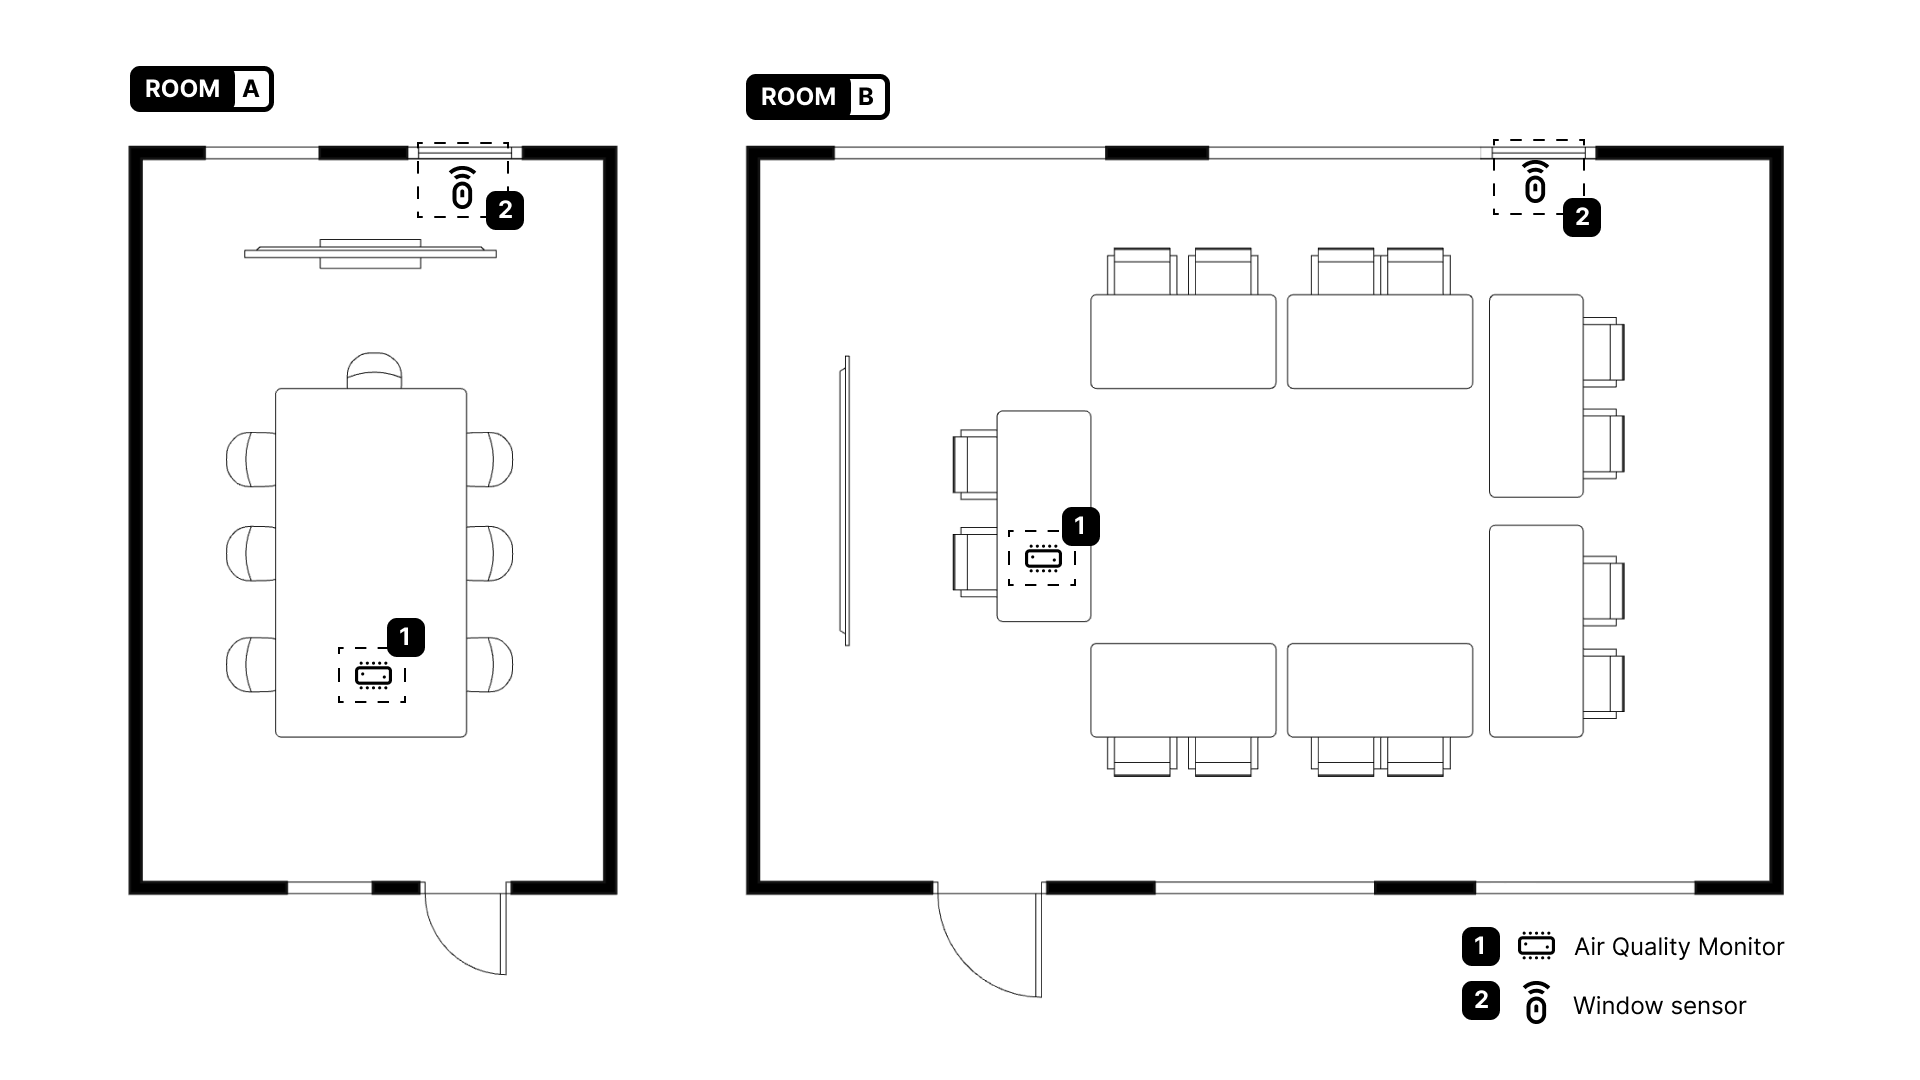
\includegraphics[width=0.8\paperwidth]{floorplan.png}
    \caption{Floorplan of Room A and B with the position of the monitor devices installed to manufacturer specifications}
    \label{fig:timeline}
\end{figure}

\section{Meeting room impressions}
\label{appendix:meetings}

Photographs of the meeting rooms used for the lab-setup.

\begin{figure}[H]
\begin{minipage}{.5\textwidth}
    \centering
    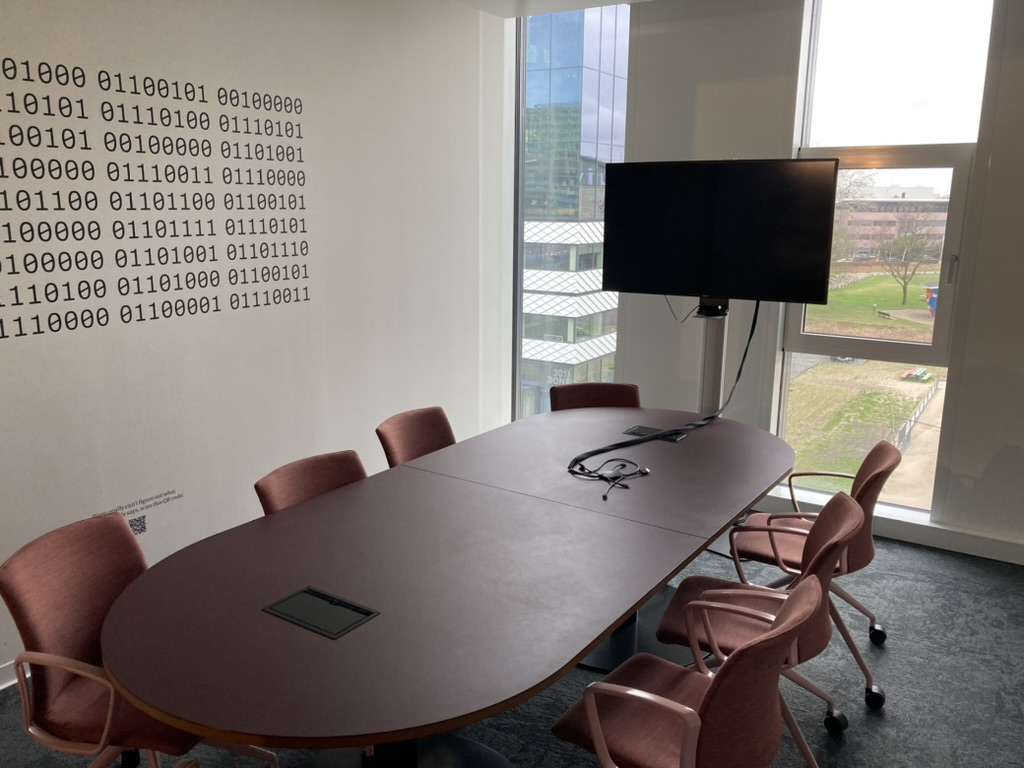
\includegraphics[width=85mm,height=70mm]{photograph-room-a.jpeg}
    \caption{The 'smaller'($m2$) space labeled Room A}
    \label{fig:timeline}
\end{minipage}%
\begin{minipage}{.5\textwidth}
    \centering
    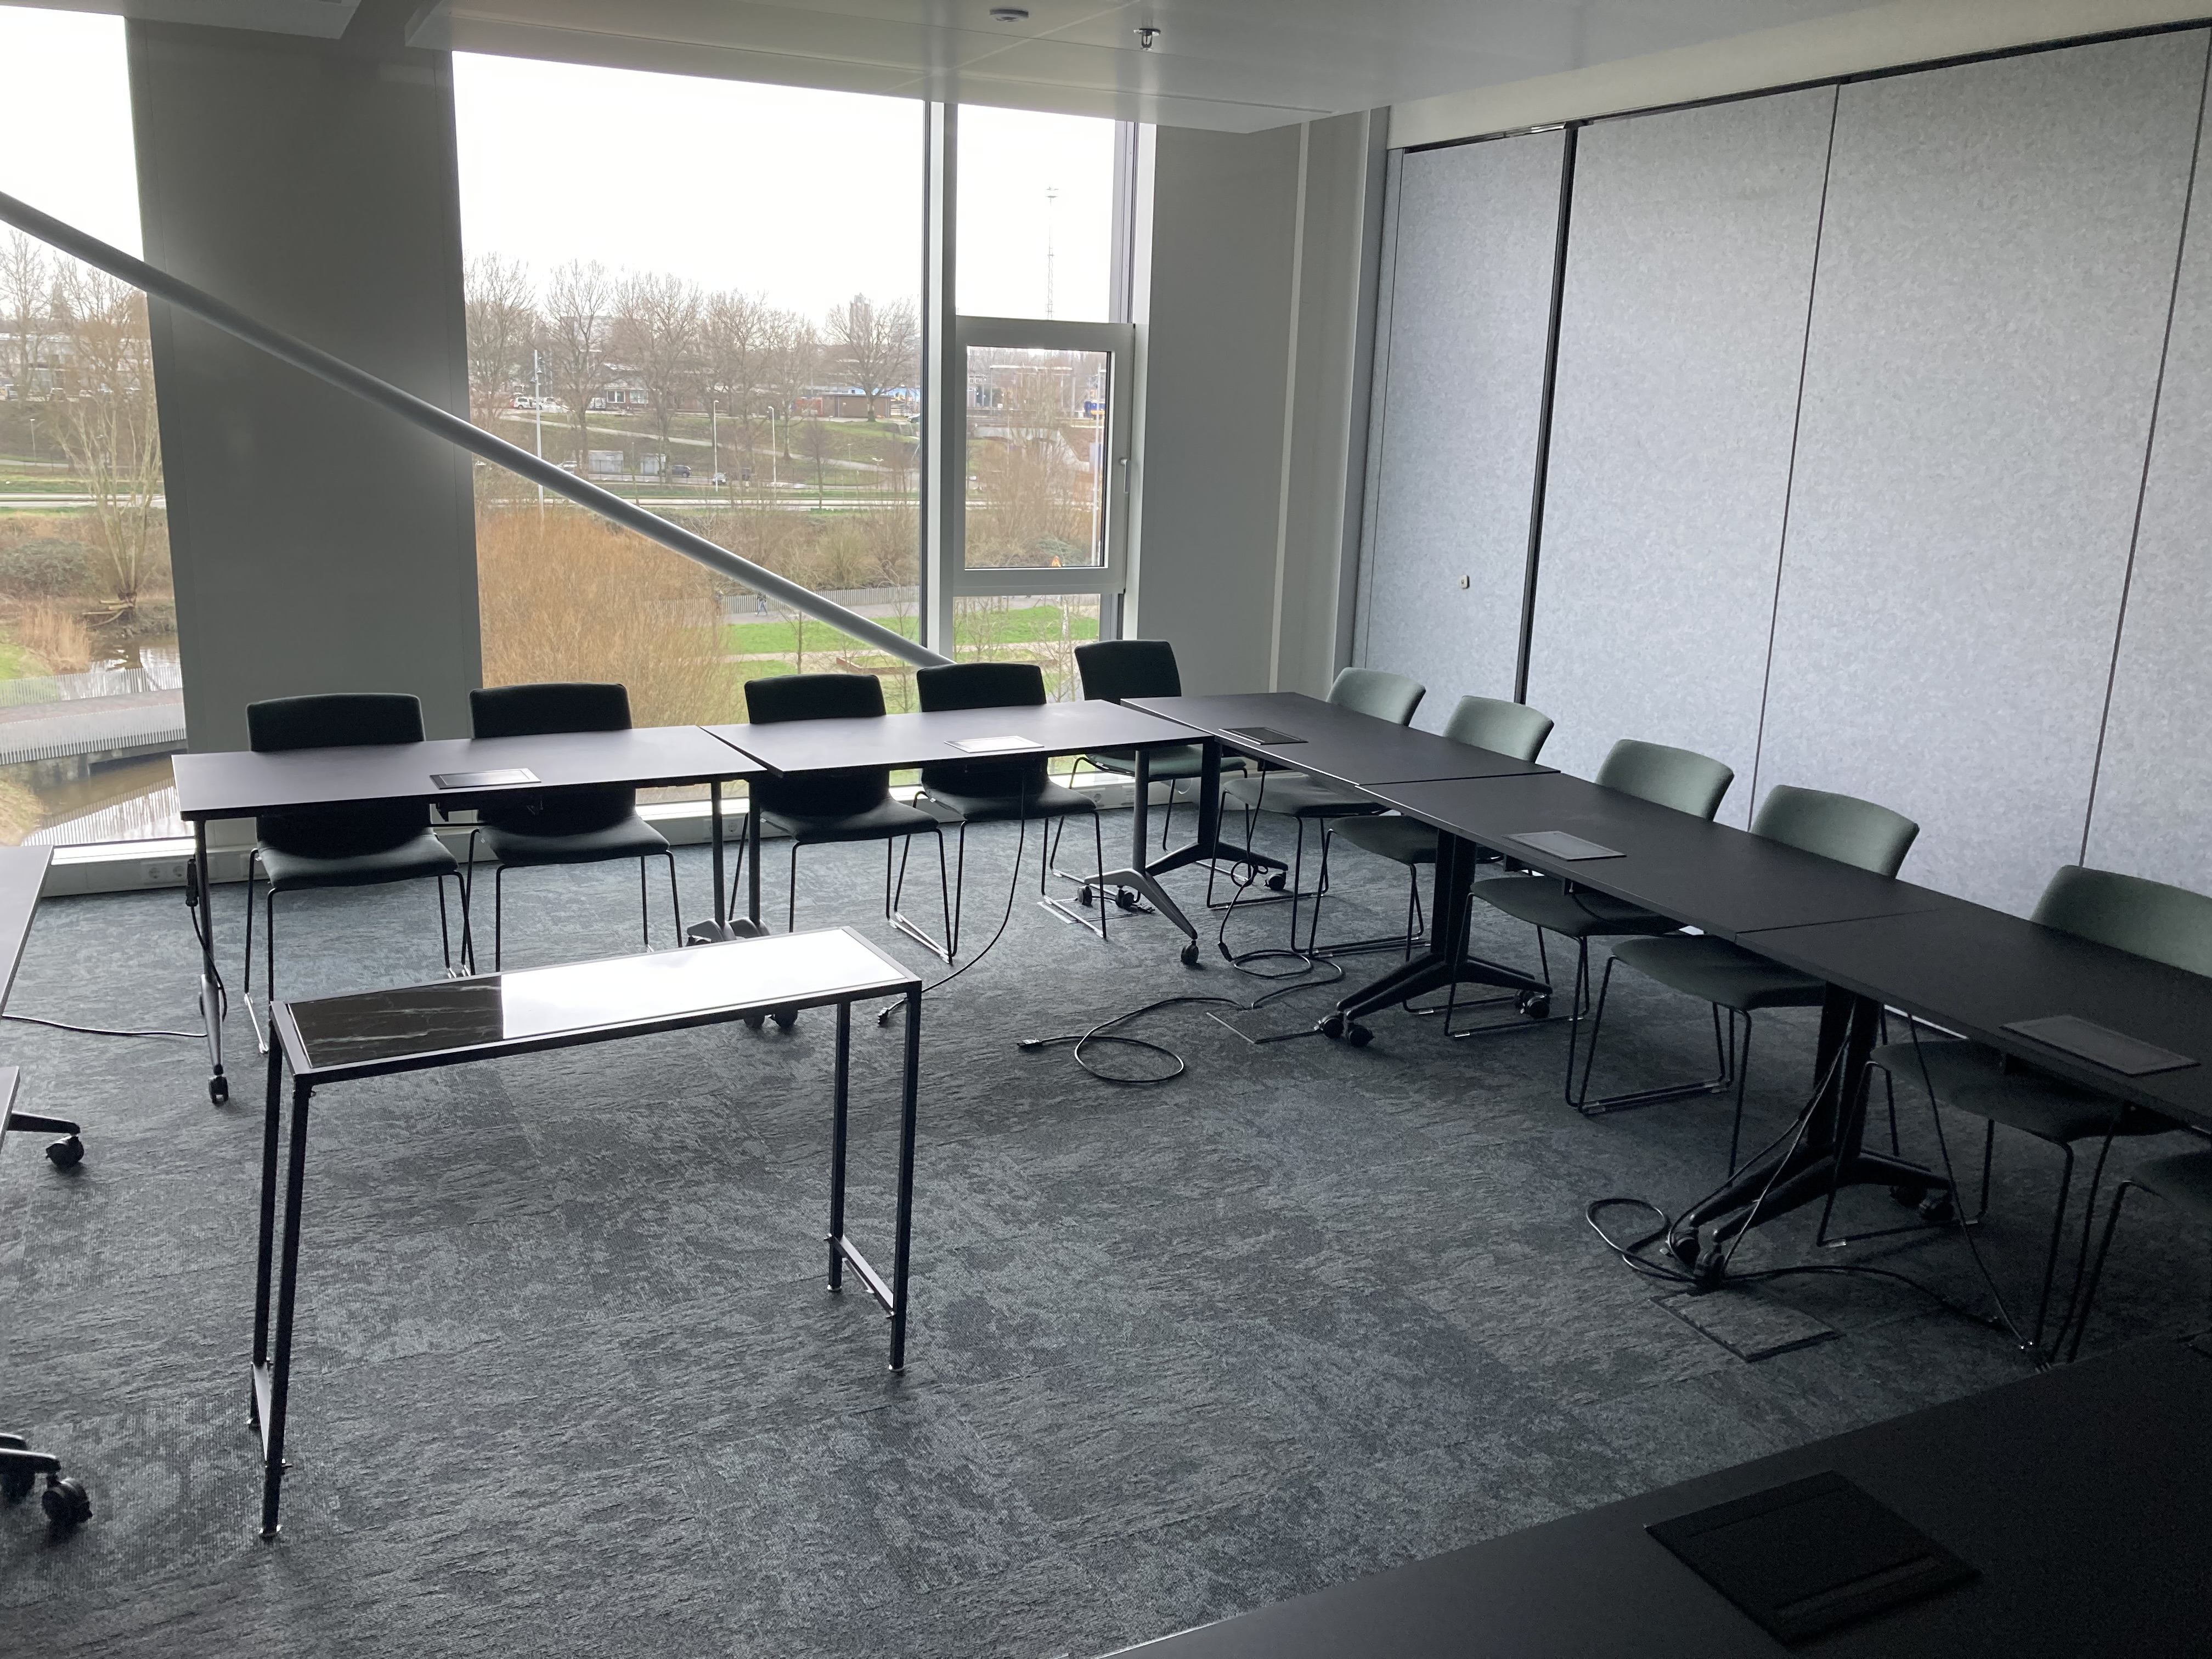
\includegraphics[width=85mm,height=70mm]{photograph-room-b.jpeg}
    \caption{The 'larger' ($m2$) space labeled Room B}
    \label{fig:timeline}
\end{minipage}%
\end{figure}

\section{Building impressions}
\label{appendix:building}

\begin{figure}[H]
\begin{minipage}{.5\textwidth}
\begin{tabular}{cc}
  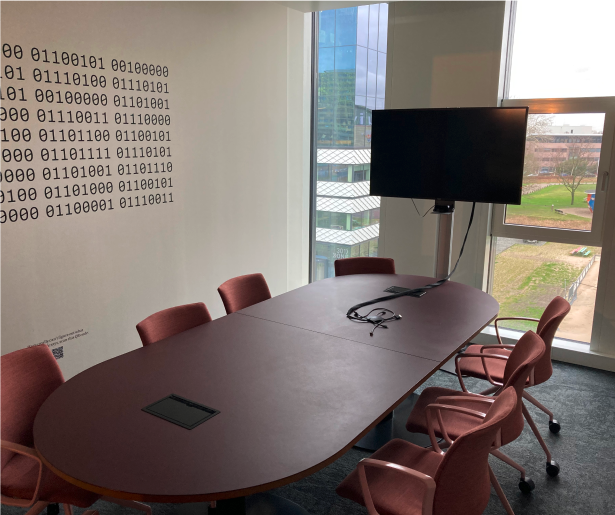
\includegraphics[width=45mm]{building.png} &   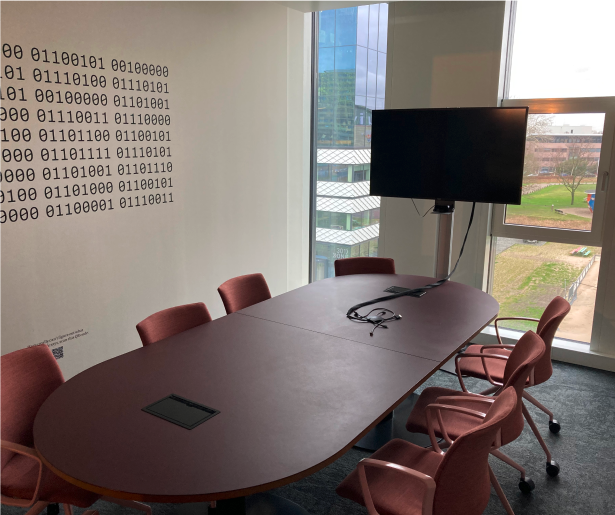
\includegraphics[width=45mm]{building.png} \\
(a) first & (b) second \\[6pt]
 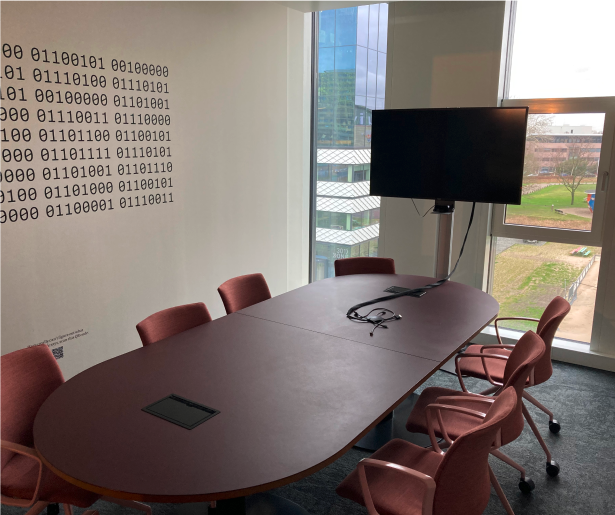
\includegraphics[width=45mm]{building.png} &   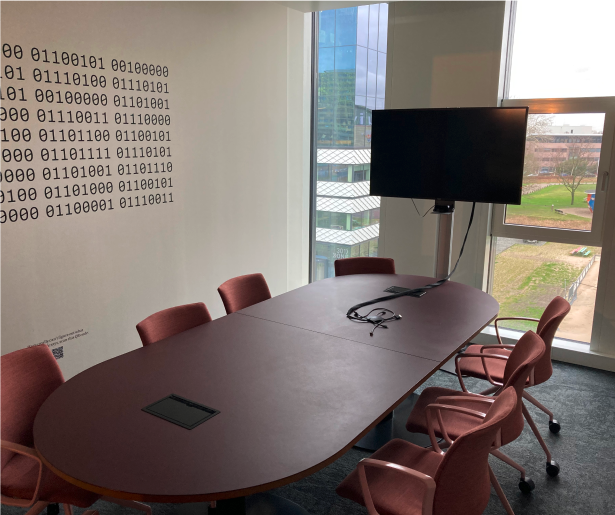
\includegraphics[width=45mm]{building.png} \\
(c) third & (d) fourth \\[6pt]
\end{tabular}
\caption{caption}
\end{minipage}%
\begin{minipage}{.5\textwidth}
    \centering
    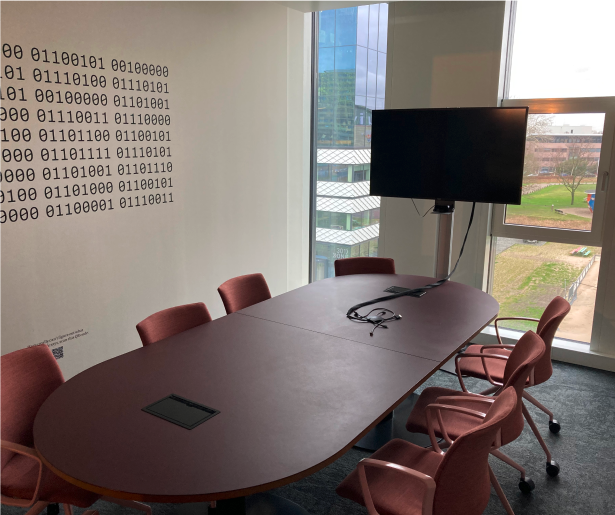
\includegraphics[width=70mm,height=80mm]{building.png}
    \caption{System diagram that shows the }
    \label{fig:timeline}
\end{minipage}%
\end{figure}

\section{Prototype impressions}
\label{appendix:prototype}

\begin{figure}[H]
\begin{minipage}{.5\textwidth}
    \centering
    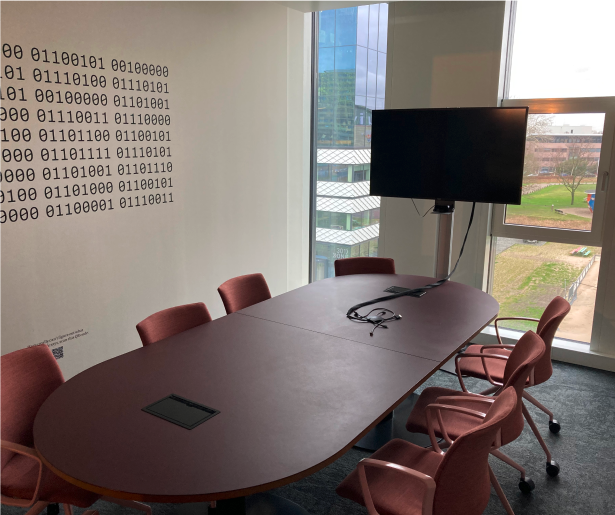
\includegraphics[width=70mm,height=80mm]{building.png}
    \caption{System diagram that shows the }
    \label{fig:timeline}
\end{minipage}%
\begin{minipage}{.5\textwidth}
\begin{tabular}{cc}
  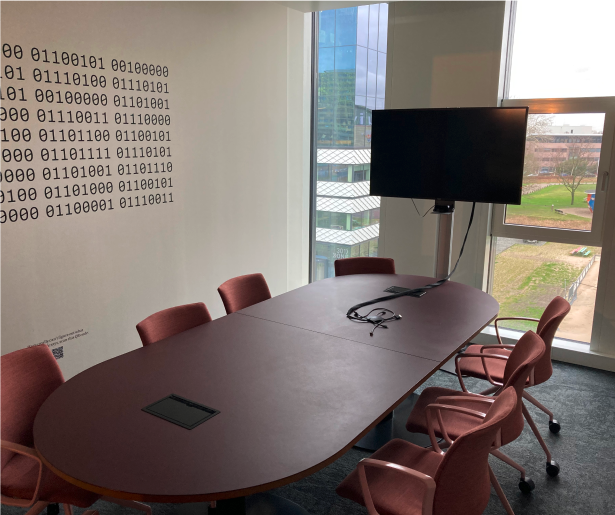
\includegraphics[width=45mm]{building.png} &   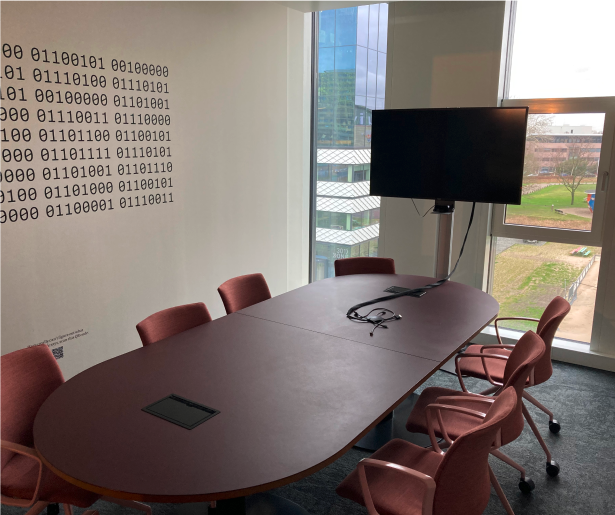
\includegraphics[width=45mm]{building.png} \\
(a) first & (b) second \\[6pt]
 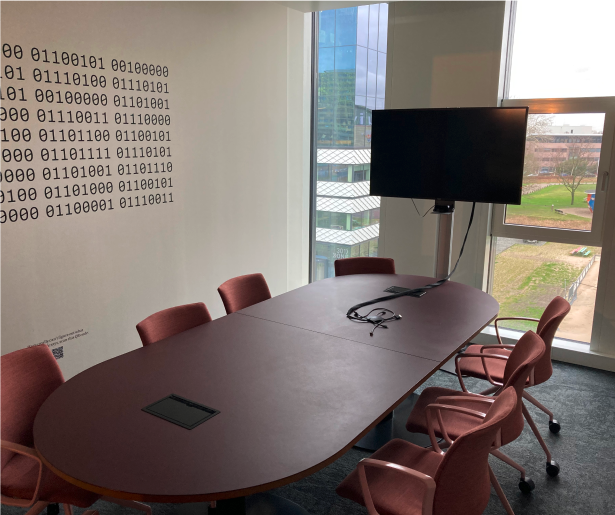
\includegraphics[width=45mm]{building.png} &   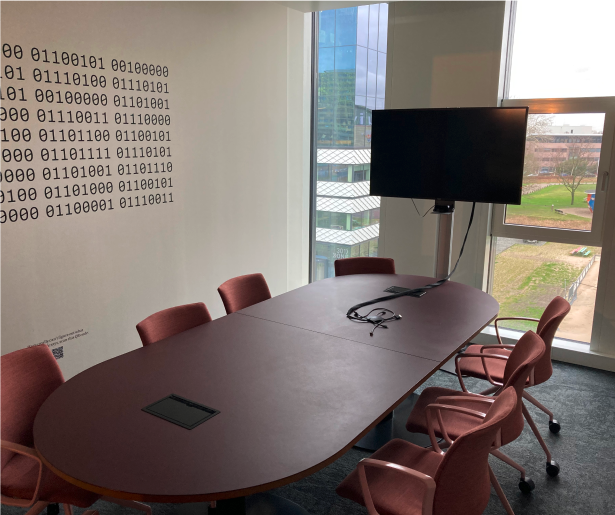
\includegraphics[width=45mm]{building.png} \\
(c) third & (d) fourth \\[6pt]
\end{tabular}
\caption{caption}
\end{minipage}%
\end{figure}

\section{IoT architecture of the prototype}
\label{appendix:architecture}

System diagram which shows the IoT architecture of the prototype.

\begin{figure}[H]
    \centering
    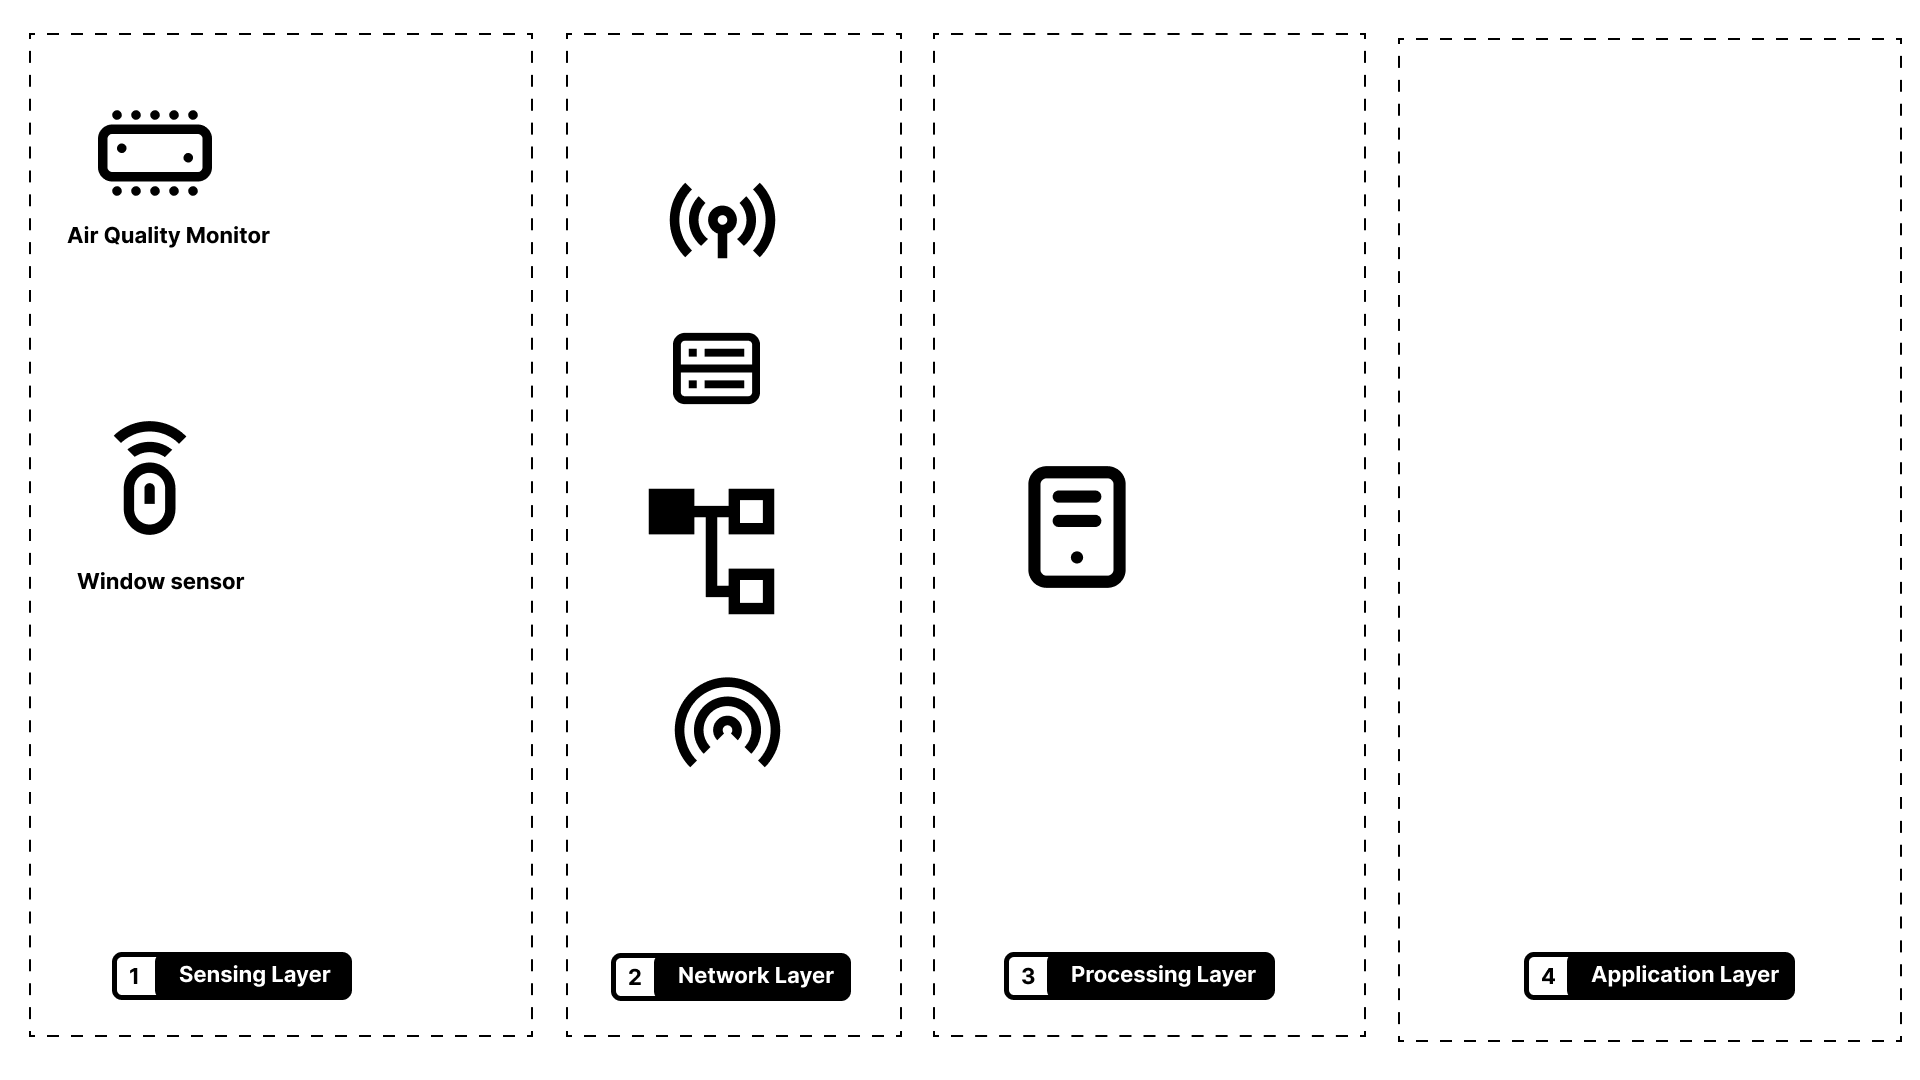
\includegraphics[width=0.7\paperwidth]{system.png}
    \caption{System diagram that shows the technical set-up of the prototype}
    \label{fig:timeline}
\end{figure}

\section{Existing Building API sample data}
\label{appendix:architecture}

Overview of the current building API with outputs.

\begin{figure}[H]
    \centering
    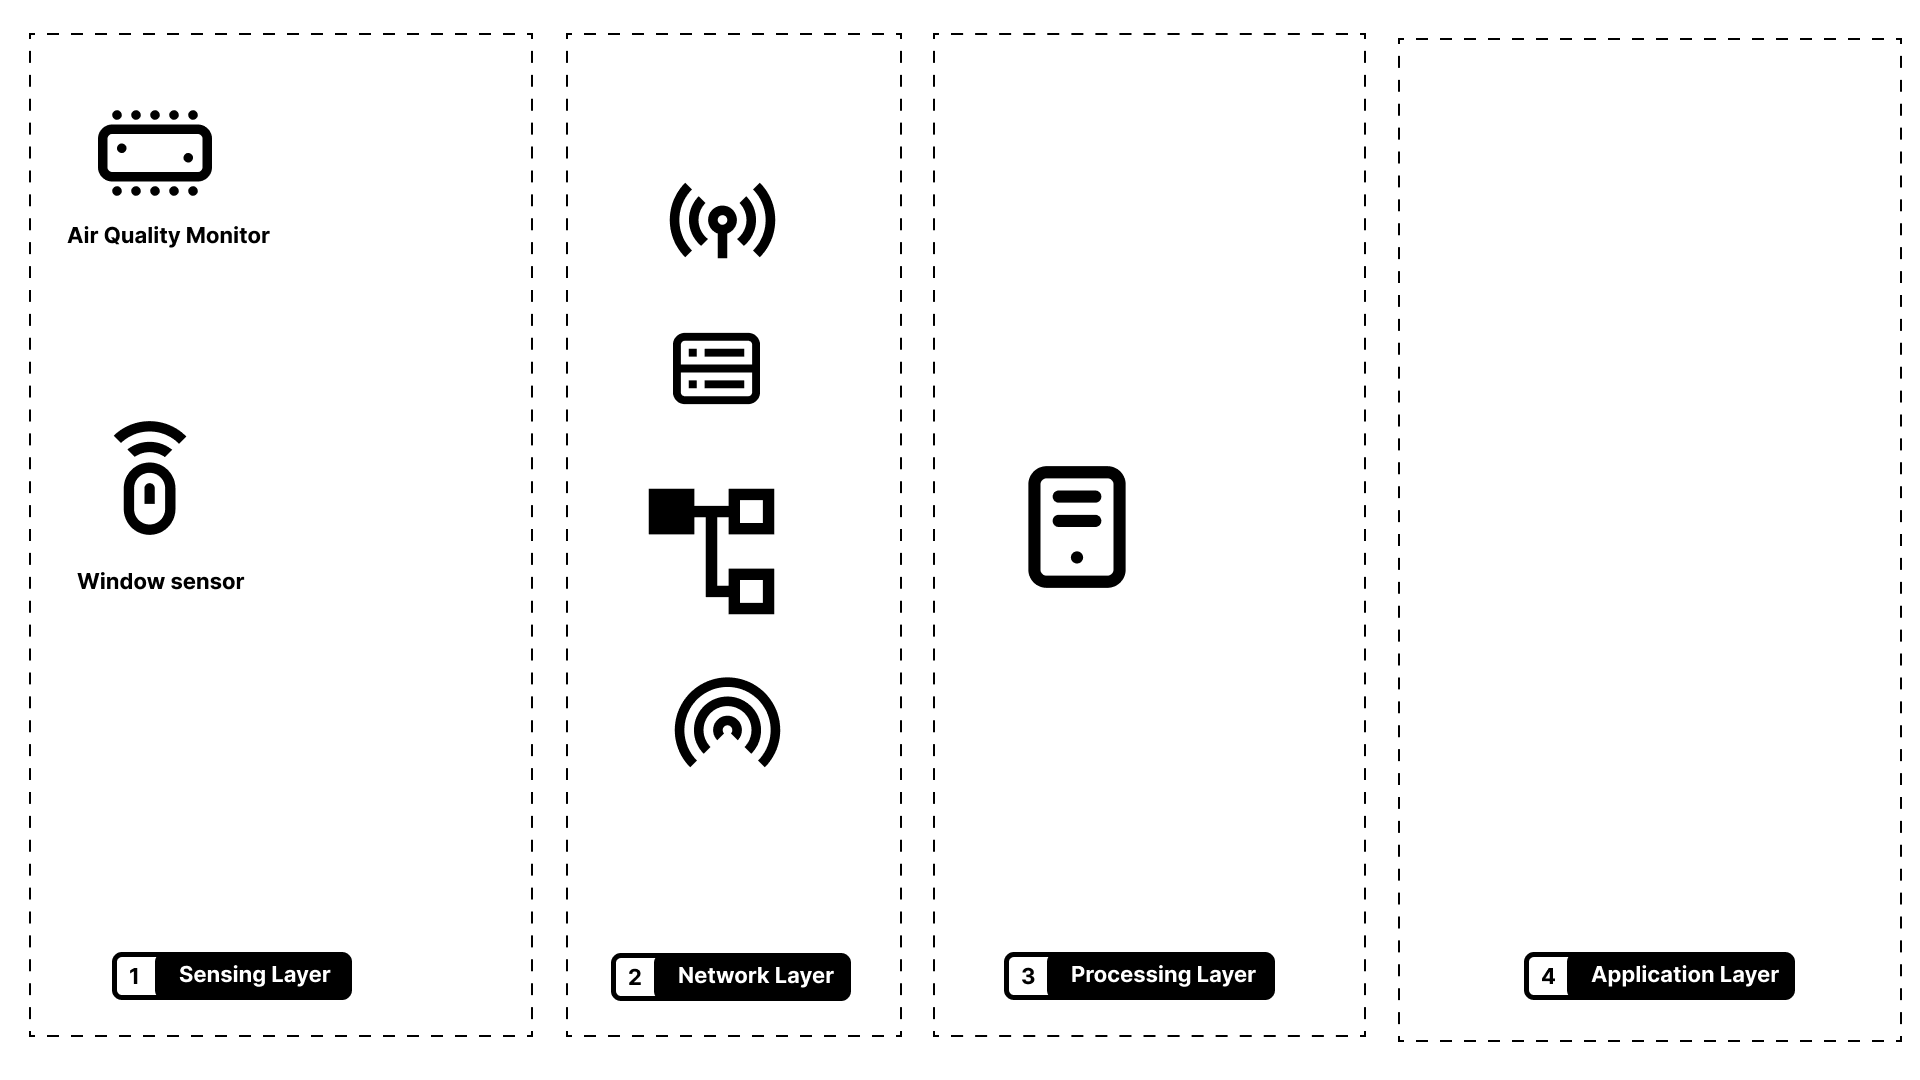
\includegraphics[width=0.7\paperwidth]{system.png}
    \caption{System diagram that shows the technical set-up of the prototype}
    \label{fig:timeline}
\end{figure}

\section{Air Quality Monitors sample data}
\label{appendix:monitors}

Sample data log of the monitor devices.

\begin{table}[H]
    \centering
    \resizebox{\textwidth}{!}{%
    \tiny
    \begin{tabular}{@{} *{11}{c} @{}}
        \toprule
        \textbf{Date} & \textbf{Time} & \textbf{CO2} & \textbf{Temp} & \textbf{RH} & \textbf{PM1.0} & \textbf{PM2.5} & \textbf{PM10} & \textbf{TVOC} & \textbf{BP} & \textbf{O3} \\
        \midrule
        2024/04/03 & 10:30 & 647 & 21'C & 39\% & 0 & 0 & 0 & 255 & 99.97 & 0 \\
        2024/04/03 & 10:29 & 641 & 21'C & 39\% & 0 & 0 & 0 & 249 & 99.97 & 0 \\
        2024/04/03 & 10:28 & 633 & 21'C & 39\% & 0 & 0 & 0 & 246 & 99.97 & 0 \\
        2024/04/03 & 10:27 & 635 & 21'C & 39\% & 1 & 1 & 1 & 242 & 99.97 & 0 \\
        2024/04/03 & 10:26 & 632 & 21'C & 39\% & 0 & 1 & 1 & 237 & 99.97 & 0 \\
        2024/04/03 & 10:25 & 628 & 21'C & 39\% & 0 & 1 & 1 & 236 & 99.97 & 0 \\
        2024/04/03 & 10:24 & 617 & 21'C & 39\% & 0 & 1 & 1 & 232 & 99.97 & 0 \\
        2024/04/03 & 10:23 & 602 & 21'C & 39\% & 0 & 1 & 1 & 232 & 99.97 & 0 \\
        2024/04/03 & 10:22 & 598 & 21'C & 39\% & 0 & 0 & 0 & 231 & 99.97 & 0 \\
        2024/04/03 & 10:21 & 591 & 21'C & 39\% & 0 & 1 & 1 & 228 & 99.97 & 0 \\
        2024/04/03 & 10:20 & 587 & 21'C & 39\% & 0 & 0 & 0 & 228 & 99.97 & 0 \\
        2024/04/03 & 10:19 & 580 & 21'C & 39\% & 0 & 0 & 0 & 230 & 99.97 & 0 \\
        2024/04/03 & 10:18 & 580 & 21'C & 39\% & 0 & 0 & 0 & 232 & 99.97 & 0 \\
        2024/04/03 & 10:17 & 578 & 21'C & 39\% & 1 & 1 & 1 & 234 & 99.97 & 0 \\
        2024/04/03 & 10:16 & 574 & 21'C & 39\% & 0 & 0 & 0 & 237 & 99.97 & 0 \\
        2024/04/03 & 10:15 & 569 & 21'C & 39\% & 0 & 0 & 0 & 237 & 99.97 & 0 \\
        \bottomrule
    \end{tabular}%
    }
    \vspace{10pt} % Adjust the amount of whitespace as needed
    \caption{Sample data log of the Aircheq Touch Aero installed in the 'small' Room A} 
    \label{tab:room-A}
\end{table}

\begin{table}[H]
    \centering
    \resizebox{\textwidth}{!}{%
    \tiny
    \begin{tabular}{@{} *{11}{c} @{}}
        \toprule
        \textbf{Date} & \textbf{Time} & \textbf{Temp} & \textbf{RH} & \textbf{DewPoint} & \textbf{CO2} & \textbf{-} & \textbf{-} & \textbf{-} & \textbf{-} & \textbf{-} \\
        \midrule
        10/04/2024 & 14:17:00 & 21.019 & 30.780 & 3.176 & 871.000 \\
        10/04/2024 & 14:18:00 & 21.039 & 30.573 & 3.098 & 871.000 \\
        10/04/2024 & 14:19:00 & 21.019 & 30.365 & 2.985 & 827.000 \\
        10/04/2024 & 14:20:00 & 21.049 & 30.164 & 2.917 & 808.000 \\
        10/04/2024 & 14:21:00 & 21.059 & 29.895 & 2.838 & 808.000 \\
        10/04/2024 & 14:22:00 & 21.059 & 29.852 & 2.772 & 773.000 \\
        10/04/2024 & 14:23:00 & 21.059 & 29.730 & 2.723 & 773.000 \\
        10/04/2024 & 14:24:00 & 21.079 & 29.608 & 2.665 & 773.000 \\
        10/04/2024 & 14:25:00 & 21.059 & 29.486 & 2.607 & 721.000 \\
        10/04/2024 & 14:26:00 & 21.059 & 29.303 & 2.520 & 714.000 \\
        10/04/2024 & 14:27:00 & 21.049 & 29.242 & 2.482 & 714.000 \\
        10/04/2024 & 14:28:00 & 21.079 & 29.181 & 2.479 & 714.000 \\
        10/04/2024 & 14:29:00 & 21.059 & 29.016 & 2.400 & 681.000 \\
        10/04/2024 & 14:30:00 & 21.089 & 28.912 & 2.358 & 681.000 \\
        \bottomrule
    \end{tabular}%
    }\vspace{10pt} % Adjust the amount of whitespace as needed
    \caption{Sample data log of the Atal ATU-CT ClimaTrend installed in the 'large' Room B} 
    \label{tab:room-b}
\end{table}


\section{Questionnaire survey (POE)}
\label{appendix:survey}

Exported text version of the questionnaire survey created in Qualtrics and distributed using handouts on QR codes.

\vspace{10pt} % Adjust the length as needed

\textbf{Introduction:}
\textit{Hi! We at the Digital Interactions Lab (DIL) are researching indoor environments, focusing on Indoor Air Quality (IAQ) within smart buildings like Lab42, for a Master Thesis. This survey takes an average of $\sim$3 minutes to complete and comprises questions about your overall comfort and awareness of Indoor Air Quality (IAQ).}\\

\textbf{Informed Consent:}
\textit{The survey is anonymous and collects data on environmental experiences and approximate building location for future research and publication. Participation is voluntary, and if you decide that you do not want to participate after you have completed it, please contact us. Principal researcher: BSc D. de Vries - danny.de.vries@student.uva.nl Supervisor(s): Shruti Rao PhD Candidate - s.rao@uva.nl Supervisor(s): Dr. H. Seiied Alavi PhD - ha.alavi@uva.nl Thank you for your valuable time and for participating in our survey!}

\vspace{10pt} % Adjust the length as needed

\textbf{Q1: Location}- Where are you currently located within the Lab42 building? \textit{Multiple-choice, one option possible}

\begin{itemize}
    \item On the ground floor (the atrium)
    \item On the first floor (1st floor - in a working space)
    \item On the second floor (2nd floor - in a working space)
\end{itemize}

\textbf{Q2: Activity} - On average, how often do you use Lab42 per week for various activities? \textit{Multiple-choice, one option possible}

\begin{itemize}
    \item 1 day a week
    \item 2 days a week
    \item 3 days a week
    \item 4 days a week
    \item 5 days a week
\end{itemize}

\textbf{Q3: Occupancy} - How would you describe the occupancy in your current space? \textit{Multiple-choice, one option possible}

\begin{itemize}
    \item Not crowded
    \item Not too crowded
    \item Crowded
    \item Very crowded
    \item At capacity
\end{itemize}

\textbf{Q4: Awareness Air Quality} - Did you know that poor air quality has been identified to pose health risks and affect cognitive performance? How aware are you of the current air quality in this space? \textit{Likert-scale, one option possible}

\textbf{1)} Very Unaware \textbf{2)} Unaware \textbf{3)} Neutral \textbf{4)} Aware \textbf{5)} Very Aware

\vspace{10pt}

\textbf{Q6: Perceived Air Quality} - How do you perceive the air quality in the current space? \textit{Likert-scale, one option possible}

\textbf{1)} Very Poor \textbf{2)} Poor \textbf{3)} Acceptable \textbf{4)} Good \textbf{5)} Very Good 

\vspace{10pt}

\textbf{Q7: Satisfaction Air Quality} - How satisfied are you with the air quality in the current space? \textit{Likert-scale, one option possible}

\textbf{1)} Very Dissatisfied \textbf{2)} Dissastisfied \textbf{3)} Neither dissatisfied or satisfied \textbf{4)} Satisfied \textbf{5)} Very Satisfied

\vspace{10pt}

\textbf{Q8: Not mandatory} - Would you like to describe in more detail in your own words how you currently feel about the Indoor Air Quality? \textit{Open-question, insert text}

\vspace{10pt}

\textbf{Q9: Health symptoms} - Do you experience any health-related symptoms based on the air quality in this space? \textit{Multiple-choice, multiple options possible, insert text field}

\begin{itemize}
    \item None
    \item Headaches
    \item Trouble breathing
    \item Feeling nauseating
    \item Other
\end{itemize}

\textbf{Q10: Cognitive symptoms} - Do you experience any cognitive-based symptoms on the air quality in this space? \textit{Multiple-choice, multiple options possible, insert text field}

\begin{itemize}
    \item None
    \item Trouble with focus
    \item Decreased productivity
    \item Tiredness
    \item Other
\end{itemize}


\section{Survey data}
\label{appendix:profile}

\section{Monitor data}
\label{appendix:profile}

\newpage

\section{Expert reviews}
\label{appendix:expert}

\section{Evaluation Interviews}
\label{appendix:evaluation}

\section{Usability tests}
\label{appendix:usability}

\section{Effectiveness scores}
\label{appendix:effectiveness}

\newpage

\section{Concept diagrams}
\label{appendix:conceptdiagrams}

Design diagrams of the brainstormed concepts in medium-fi sketches that show the component breakdown and interaction states.

\begin{figure}[H]
    \centering
    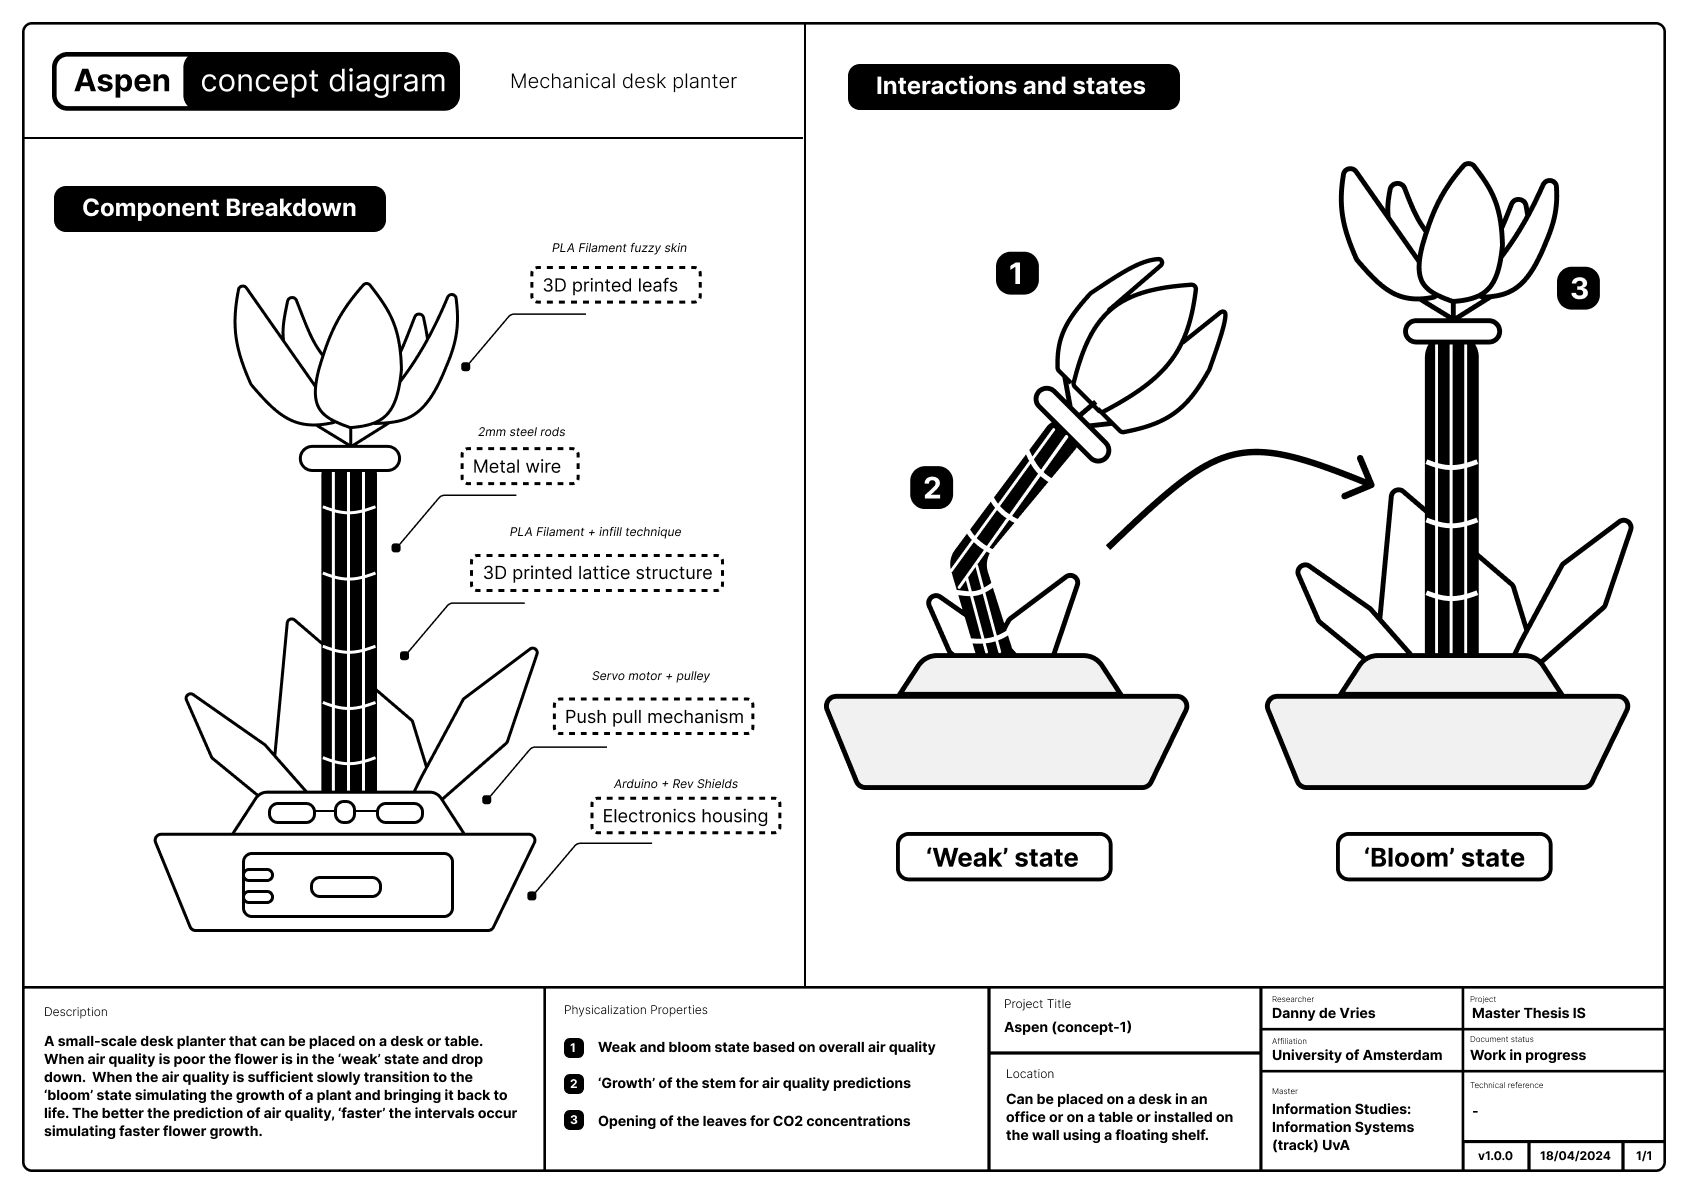
\includegraphics[width=0.6\paperwidth]{Concept-1_Aspen_Design_Diagram.jpg}
    \caption{Design diagram of Concept-2}
    \label{fig:timeline}
\end{figure}

\begin{figure}[H]
    \centering
    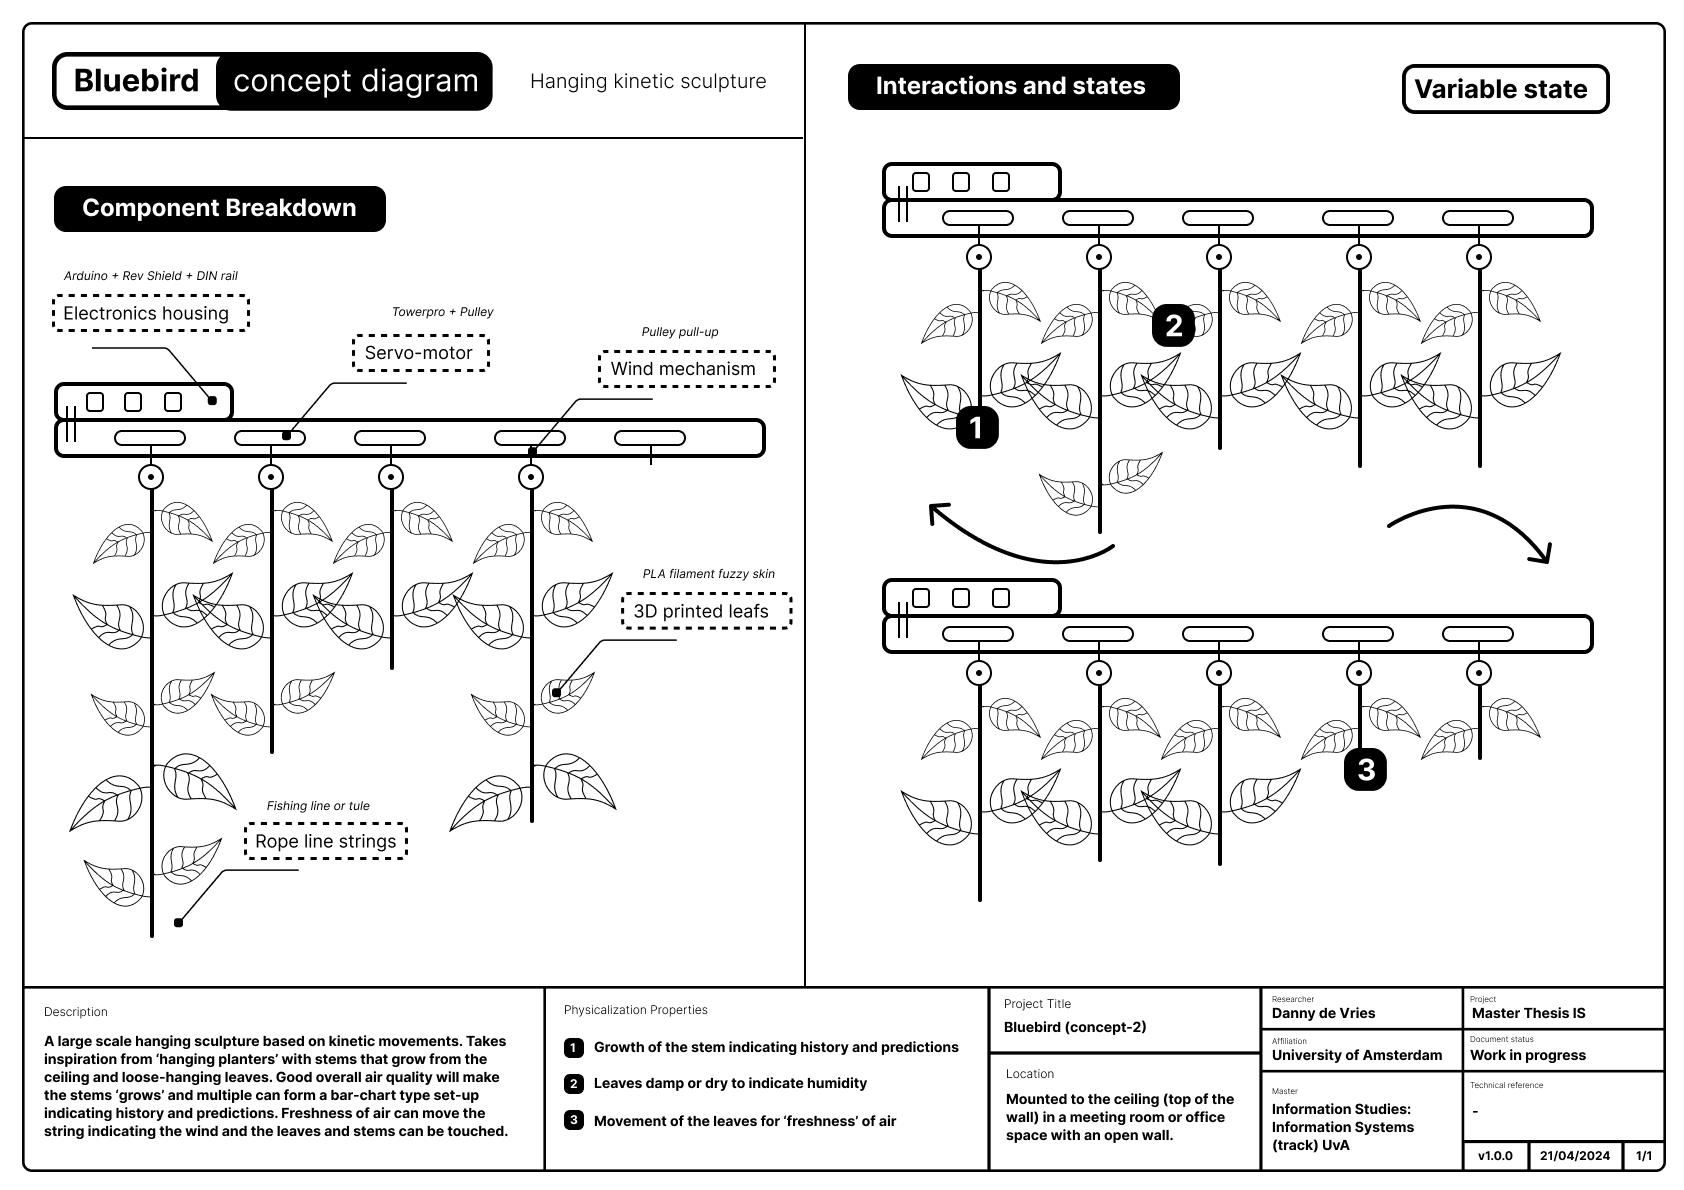
\includegraphics[width=0.6\paperwidth]{Concept-2_Bluebird_Design_Diagram.jpg}
    \caption{Design diagram of Concept-2}
    \label{fig:timeline}
\end{figure}

\begin{figure}[H]
    \centering
    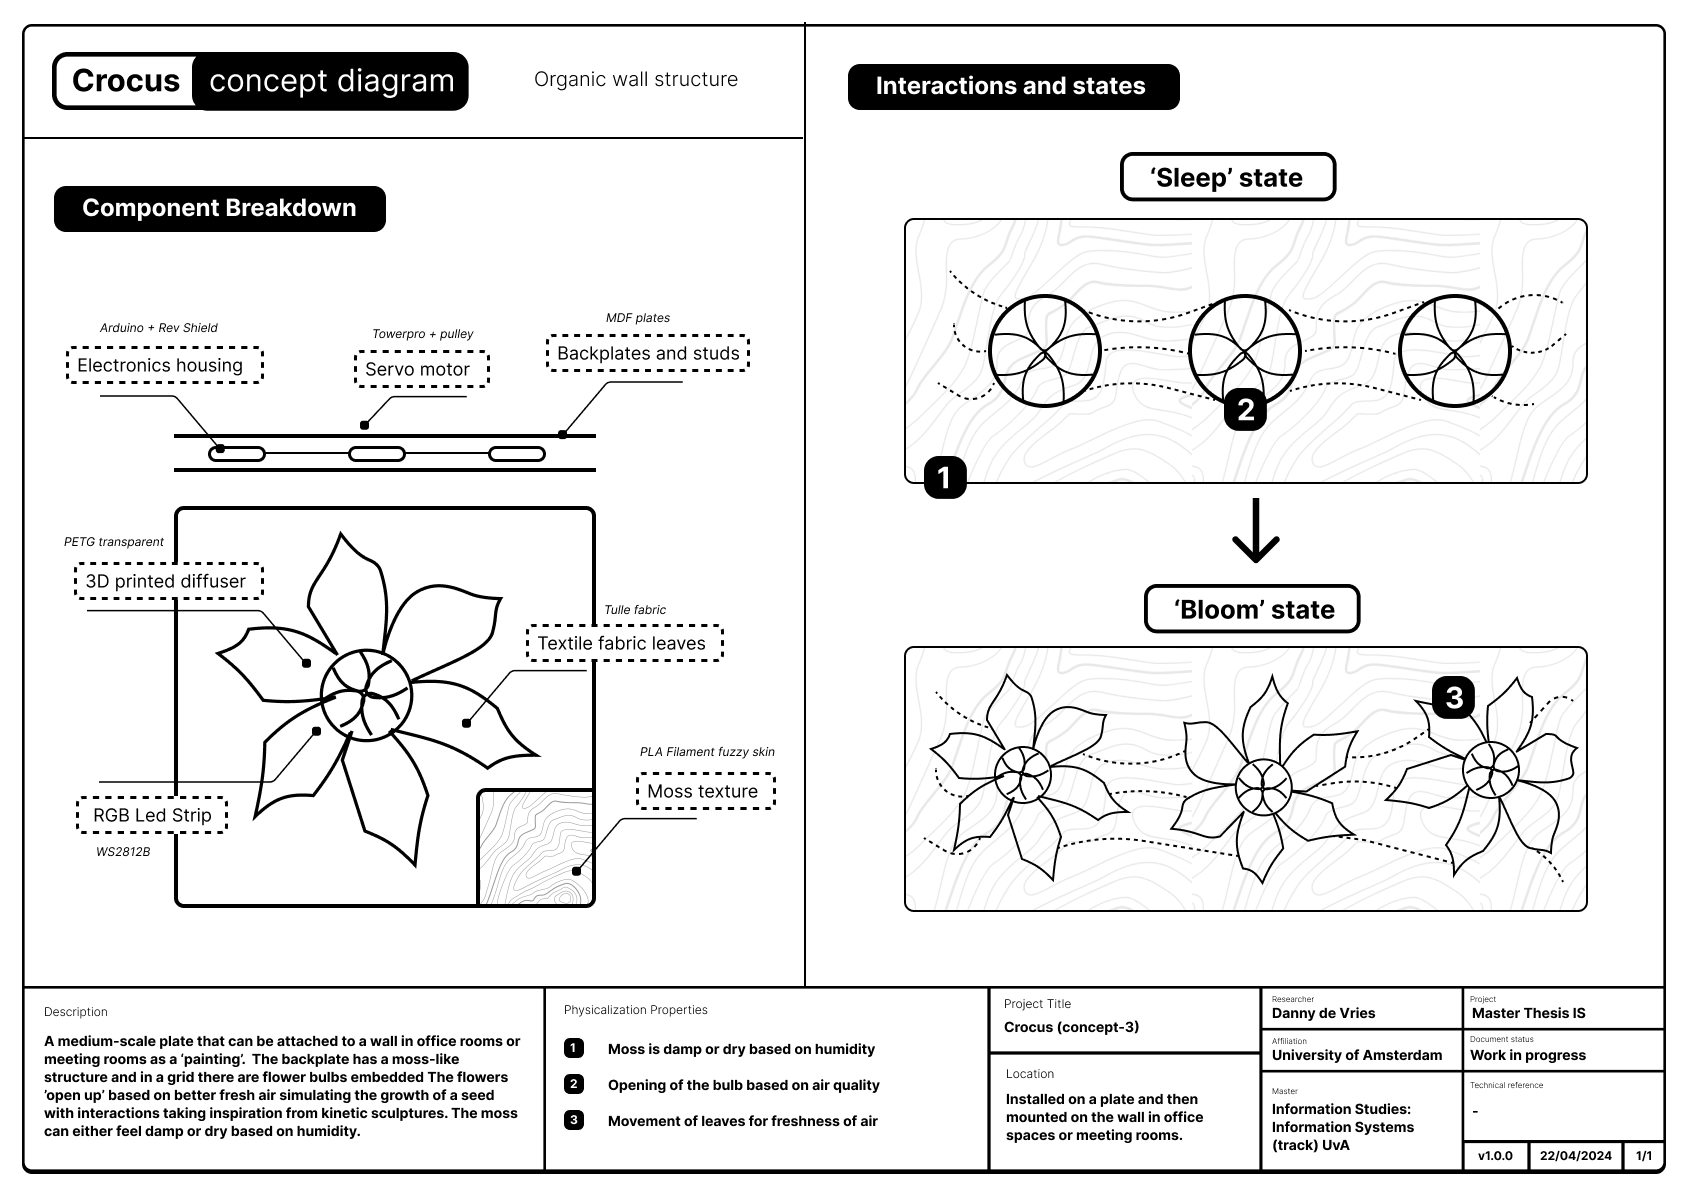
\includegraphics[width=0.6\paperwidth]{Concept-3_Crocus_Design_Diagram.jpg}
    \caption{Design diagram of Concept-3}
    \label{fig:timeline}
\end{figure}

\section{Academic sample case studies}
\label{appendix:academic}

In the ideation phase and development of concept models, seven academic publications were instrumental in informing and inspiring the design process. Table 1 provides an overview of these publications, presenting details such as the title, authors, publication year, and relevant venue.

\begin{table}[htbp]
\centering
\caption{Overview of the 7 academic case studies used for the ideation phase and concept models.}
\label{tab:my-table}
\begin{tabularx}{\textwidth}{|>{\raggedright\arraybackslash}m{1cm}|X|X|>{\raggedright\arraybackslash}m{1cm}|X|X|}
\hline
\textbf{Nr.} & \textbf{Sample} & \textbf{Author(s)} & \textbf{Year} & \textbf{Venue} & \textbf{Reference} \\ \hline
1 & Econundrum & Unknown & Unknown & non-academic & \href{https://dl.acm.org/doi/10.1145/3357236.3395509}{Econundrum} \\ \hline
2 & Caimform & Unknown & Unknown & non-academic & \href{http://dataphys.org/list/cairnform-a-physical-ring-chart-showing-renewable-energy-data/}{Caimform} \\ \hline
3 & Dataponics & Unknown & Unknown & non-academic & \href{http://dataphys.org/list/dataponics-human-vegetal-play/}{Dataponics} \\ \hline
4 & Garden of Eden & Unknown & Unknown & non-academic & \href{http://dataphys.org/list/garden-of-eden/}{Garden of Eden} \\ \hline
5 & Pudica & Unknown & Unknown & non-academic & \href{https://trackr-media.tangiblemedia.org/publishedmedia/Papers/715-MTA0N/Published/PDF}{Pudica} \\ \hline
6 & ComfortBox & Hamed S. Alavi et al. & 2017 & IFIP & \href{https://doi.org/10.1007/978-3-319-67687-6_16}{ComfortBox} 
\\ \hline
7 & ComFeel & Ugo Sassi et al. & 2020 & ACM & \href{https://dl.acm.org/doi/10.1145/3432234}{ComFeel} 
\\ \hline
8 & WindowWall & Patrick Bader et al. & 2020 & ACM & \href{https://doi.org/10.1145/3310275}{WindowWall} \\ \hline
9 & Ambient Influence & Yvonne Rogers et al. & 2010 & ACM & \href{https://dl.acm.org/doi/10.1145/1864349.1864372}{Ambient Influence} 
\\ \hline
10 & Hilo-wear & Shailin Zong et al. & 2020 & CHI & \href{https://dl.acm.org/doi/10.1145/3334480.3382813}{Hilo-wear} 
\\ \hline
\end{tabularx}
\end{table}

\section{Non-academic sample case studies}
\label{appendix:nonacademic}

In the ideation phase and development of concept models, an exploration of non-academic case studies were instrumental in informing and inspiring the design process. Table 2 presents an overview of the 15 non-academic case studies. Each entry in the table includes essential details such as the title, creator, publication year, and a brief description of the case study's venue.

\begin{table}[htbp]
\centering
\caption{Overview of the 28 non-academic case studies used for the ideation phase and concept models.}
\label{tab:my-table}
\begin{tabularx}{\textwidth}{|>{\raggedright\arraybackslash}m{1cm}|X|X|>{\raggedright\arraybackslash}m{1cm}|X|X|}
\hline
\textbf{Nr.} & \textbf{Sample} & \textbf{Creator} & \textbf{Year} & \textbf{Venue} & \textbf{Reference} \\ \hline
1 & Birdie Design & Birdie Design & 2024 & non-academic & \href{https://www.bir.die/}{www.bir.die} \\ \hline
2 & Fields of Informality & Zhestkov & 2024 & non-academic & \href{https://www.artco.m.com/}{www.artco.m} \\ \hline
3 & Tree of Ténéré & Studio Drift & 2024 & non-academic & \href{https://studiodr.ift.com/}{www.studiodr} \\ \hline
4 & Kinetic Sculpture & ART+COM & 2024 & non-academic & \href{https://artco.m.com/}{www.artco.m} \\ \hline
5 & Electro Magnetic Field & Unknown & 2024 & non-academic & - \\ \hline
6 & Microsurgical Robot & Unknown & 2024 & non-academic & - \\ \hline
7 & Wind 3.0 & Studio Roosegaarde & 2024 & non-academic & \href{https://www.studior.oo/}{www.studior} \\ \hline
8 & Floralis Generica & Eduardo Catalano & 2024 & non-academic & - \\ \hline
9 & Lucid Stead & Phillip K. Smith III & 2024 & non-academic & - \\ \hline
10 & Flylight & Studio Drift & 2024 & non-academic & - \\ \hline
11 & Spectra 2 & FIELD & 2024 & non-academic & - \\ \hline
12 & Meadow & Studio Drift & 2024 & non-academic & - \\ \hline
13 & Wind Pavilion & Studio Roosegaarde & 2024 & non-academic & - \\ \hline
14 & Pet Lamp & Álvaro Catalán & 2024 & non-academic & - \\ \hline
15 & Living map & Unknown & Unknown & non-academic & \href{https://www.behance.net/gallery/68572509/LIVING-MAP}{Living map} \\ \hline
16 & Harassment plants & Unknown & Unknown & non-academic & \href{https://luizaugustomm.github.io/pages/harassment-plants.html}{Harassment plants} \\ \hline
17 & Popsicles of Pollution & Unknown & Unknown & non-academic & \href{https://www.theguardian.com/cities/gallery/2017/sep/01/popsicles-pollution-ice-lollies-taiwan-taipei-contaminated-waterways}{Popsicles of Pollution} \\ \hline
18 & Yellow Dust & Unknown & Unknown & non-academic & \href{http://yellowdust.intheair.es/}{Yellow Dust} \\ \hline
19 & Touching air & Unknown & Unknown & non-academic & \href{https://www.stefanieposavec.com/airtransformed}{Touching air} \\ \hline
20 & Physical Weather Display & Unknown & Unknown & non-academic & \href{https://www.boredpanda.com/weather-forecast-box-tempescope-ken-kawamoto/}{Physical Weather Display} \\ \hline
21 & Inequalities Quipu & Unknown & Unknown & non-academic & \href{https://tuteja.info/inequalities-quipu/}{Inequalities Quipu} \\ \hline
22 & Summer in the city & Unknown & Unknown & non-academic & \href{https://www.carolabartsch.ch/en/projects/dataviz}{Summer in the city} \\ \hline
23 & WeatherWindow & Unknown & Unknown & non-academic & \href{http://dataphys.org/list/weatherwindow/}{WeatherWindow} \\ \hline
24 & Point cloud & Unknown & Unknown & non-academic & \href{https://www.jamesleng.net/pointcloud/}{Point cloud} \\ \hline
25 & Tele-present water & Unknown & Unknown & non-academic & \href{https://www.dwbowen.com/telepresentwater/}{Tele-present water} \\ \hline
26 & Real-time Warning & Unknown & Unknown & non-academic & \href{https://vimeo.com/35520114}{Real-time Warning} \\ \hline
27 & airFIELD & Unknown & Unknown & non-academic & \href{http://dataphys.org/list/ecloud-airfield-ambient-airport-visualizations/}{airFIELD} \\ \hline
28 & Shanghai Spheres & Unknown & Unknown & non-academic & \href{https://www.taittowers.com/work?sort=newest}{Shanghai Spheres} \\ \hline
\end{tabularx}
\end{table}

\section{fabrication Techniques}
\label{appendix:fabrication}

\begin{table}[!htbp]
\centering
\caption{Overview of the 4 academic and 6 non-academic sample case studies used as inspiration for fabrication of the prototype.}
\label{tab:my-table}
\begin{tabularx}{\textwidth}{|>{\raggedright\arraybackslash}m{1cm}|X|X|>{\raggedright\arraybackslash}m{1cm}|X|X|}
\hline
\textbf{Nr.} & \textbf{Sample} & \textbf{Author(s)} & \textbf{Year} & \textbf{Venue} & \textbf{Reference} \\ \hline
1 & FibeRobo & Jack Forman et al. & 2023 & MIT Media Lab (TGM) & \href{https://trackr-media.tangiblemedia.org/publishedmedia/Papers/728-MTA2O/Published/PDF}{TGM} \\ \hline
2 & DefeXtiles & Jack Forman et al. & 2020 & MIT Media Lab (TGM) & \href{https://trackr-media.tangiblemedia.org/publishedmedia/Papers/703-MTAyN/Published/PDF}{TGM} \\ \hline
3 & Cilllia & Jifei Ou et al. & 2016 & MIT Media Lab (TGM) & \href{https://trackr-media.tangiblemedia.org/publishedmedia/Papers/703-MTAyN/Published/PDF}{TGM} \\ \hline
4 & UniMorph & Felix Heiberg et al. & 2015 & MIT Media Lab (TGM) & \href{https://trackr-media.tangiblemedia.org/publishedmedia/Papers/703-MTAyN/Published/PDF}{TGM} \\ \hline
5 & Geometric Floating Fabric & Billie Ruben & 2020 & non-academic & \href{https://www.printables.com/en/model/42342-geometric-floating-fabric-printed-necklace-by-bill}{Printables} \\ \hline
6 & Print On Fabric & Damien Jorrand & 2021 & non-academic & \href{https://than.gs/m/14347}{Thangs} \\ \hline
7 & Nasa Fabric Mk3 & John Bowler & 2018 & non-academic & \href{https://www.thingiverse.com/thing:3095799}{Thingiverse} \\ \hline  
8 & Servo Flower & Job Smolders & 2018 & non-academic & \href{https://pinshape.com/items/41182-3d-printed-servo-flower}{Pinshape} \\ \hline
9 & Multiuse Flexible Fabric & Posix & 2024 & non-academic & \href{https://www.printables.com/model/88579-multiuse-flexible-fabric}{Printables} \\ \hline
10 & Leaf Decorative Holder & Trilobyte3D & 2022 & non-academic & \href{https://www.printables.com/model/230363-leaf-drink-coasters-with-decorative-plant-holder}{Printables} \\ \hline
\end{tabularx}
\end{table}

\end{appendices}

\end{document}

%%%%%%%%%%%%%%%%%%%%%%%%%%%%%%%%%%%%%%%%%%%%%%%%%%%%%%%%%%%%%%%%%%%%%%%%%%%%%%%%
%%%%%%%%%%%%%%%%%%%%%%%%%%%%%%%%%%%%%%%%%%%%%%%%%%%%%%%%%%%%%%%%%%%%%%%%%%%%%%%%